\documentclass[11pt,a4paper]{article}

% Language setting
\usepackage[english]{babel}

% Set page size and margins
% \usepackage[a4paper,top=2cm,bottom=2cm,left=2.5cm,right=2.5cm,marginparwidth=1.75cm]{geometry}
\usepackage[a4paper,top=2cm,bottom=2cm,left=2.5cm,right=2.5cm,margin=1in]{geometry}

%----------- APA style references & citations (starting) ---
% Useful packages
%\usepackage[natbibapa]{apacite} % APA-style citations.

\usepackage[style=numeric, backend=biber, sorting=ynt]{biblatex} % APA 7th edition style citations using biblatex
\addbibresource{references.bib} % Your .bib file

% Formatting DOI in APA-7 style
%\renewcommand{\doiprefix}{https://doi.org/}

% Add additional APA 7th edition requirements
% \DeclareLanguageMapping{british}{british-apa} % Set language mapping
% \DeclareFieldFormat[article]{volume}{\apanum{#1}} % Format volume number

% Modify 'and' to '&' in the bibliography
\renewcommand*{\finalnamedelim}{%
  \ifnumgreater{\value{liststop}}{2}{\finalandcomma}{}%
  \addspace\&\space}
  
%----------- APA style references & citations (ending) ---


\usepackage{amsmath}
\usepackage{graphicx}
\usepackage[colorlinks=true, allcolors=blue]{hyperref}
\usepackage{hyperref}
%\usepackage{orcidlink}
\usepackage[title]{appendix}
\usepackage{mathrsfs}
\usepackage{amsfonts}
\usepackage{booktabs} % For \toprule, \midrule, \botrule
\usepackage{caption}  % For \caption
\usepackage{threeparttable} % For table footnotes
\usepackage{algorithm}
\usepackage{algorithmicx}
\usepackage{algpseudocode}
\usepackage{listings}
\usepackage{enumitem}
\usepackage{chngcntr}
\usepackage{booktabs}
\usepackage{lipsum}
\usepackage{subcaption}
\usepackage{authblk}
\usepackage[T1]{fontenc}    % Font encoding
\usepackage{csquotes}       % Include csquotes
\usepackage{diagbox}


% Customize line spacing
\usepackage{setspace}
% \onehalfspacing % 1.5 line spacing

% Redefine section and subsection numbering format
\usepackage{titlesec}
\titleformat{\section} % Redefine section numbering format
  {\normalfont\Large\bfseries}{\thesection.}{1em}{}
  
% Customize line numbering format to right-align line numbers
% \usepackage{lineno} % Add the lineno package
% \renewcommand\linenumberfont{\normalfont\scriptsize\sffamily\color{blue}}
% \rightlinenumbers % Right-align line numbers

% \linenumbers % Enable line numbering

% Define a new command for the fourth-level title.
\newcommand{\subsubsubsection}[1]{%
  \vspace{\baselineskip}% Add some space
  \noindent\textbf{#1\\}\quad% Adjust formatting as needed
}
% Change the position of the table caption above the table
\usepackage{float}   % for customizing caption position
\usepackage{caption} % for customizing caption format
% \captionsetup[table]{position=top} % caption position for tables

% Define the unnumbered list
\makeatletter
\newenvironment{unlist}{%
  \begin{list}{}{%
    \setlength{\labelwidth}{0pt}%
    \setlength{\labelsep}{0pt}%
    \setlength{\leftmargin}{2em}%
    \setlength{\itemindent}{-2em}%
    \setlength{\topsep}{\medskipamount}%
    \setlength{\itemsep}{3pt}%
  }%
}{%
  \end{list}%
}
\makeatother

% Suppress the warning about \@parboxrestore
\pdfsuppresswarningpagegroup=1


%-------------------------------------------
% Paper Head
%-------------------------------------------
\title{Comparison between Distributed Locking Service Implemented on Raft and Simple Paxos  }

\author[1]{Junkai Liang}
\author[1]{Chieh Nien}
\affil[1]{\small Computer Science Department, Viterbi School of Engineering, University of Southern California}

\date{}  % Remove date

\begin{document}
\maketitle

\begin{abstract}
% Abstracts must be able to stand alone and so cannot contain citations to the paper’s references, equations, etc. An abstract must consist of a single paragraph and be concise. Because of online formatting, abstracts must appear as plain as possible. Three to six keywords must be included. Each keyword should not exceed three words. %\lipsum[1]

\end{abstract}
We implemented a distributed locking service based on a distributed key-value store, using different consensus algorithms (Raft and Simple Paxos) at the core. We conducted a comparison of performance, scalability, and fault tolerance between our distributed locking service running on Raft and Paxos to understand the impact of consensus protocols and the differences between Raft and Paxos. Using the same upper-level key-value store implementation for the locking service, the Raft-based version consistently outperformed the Paxos-based version in all aspects. We believe this is due to three main reasons: 1) Raft's strong leader structure is more compatible with the locking service scenario; 2) Raft requires only one bidirectional communication between the leader and followers, whereas Paxos requires three for each decided operation; 3) Raft can batch several operations at once, while Simple Paxos needs to send each operation individually.

\textbf{Keywords}: Locking Service, Distributed System, Raft, Paxos, Network.

%-------------------------------------------
% Paper Body
%-------------------------------------------
%--- Section ---%
\section{Overview}

% Your introduction goes here! Simply start writing your document and use the Recompile button to view the updated PDF preview. Examples of commonly used commands and features are listed below to help you get started.
% \lipsum[2]

% Once familiar with the editor, you can find various project settings in the Overleaf menu, accessed via the button at the top left of the editor. To view tutorials, user guides, and further documentation, please visit our \href{https://www.overleaf.com/learn}{help library}, or head to our plans page to \href{https://www.overleaf.com/user/subscription/plans}{choose your plan}. 

% This is an example of a new paragraph with a numbered footnote\footnote{\url{https://data.gov.uk/}} and a second footnote marker.\footnote{Example of footnote text.}
The evolution of distributed systems has been characterized by the growing complexity of modern applications and the demand for scalable, reliable, and fault-tolerant infrastructure. Distributed systems have transitioned from simple client-server architectures to highly distributed and decentralized environments, driven by the needs of web-scale applications and cloud computing.In this context, robust coordination and synchronization mechanisms have become a pivotal component in the distributed systems landscape.

However, locks or mutexes that work well on single machines often face significant challenges when applied to distributed systems.
Intrigued by this problem, we explored it further. Our research led us to Chubby \cite{burrows2006chubby}, a locking service developed by Google in 2006 to ensure that multiple processes running on different machines could coordinate effectively . At the time, the predominant consensus algorithm was Paxos \cite{lamport1998paxos,lamport2001paxos}, introduced by Leslie Lamport in 1998 . Chubby was built on an improved version of Paxos.

However, in 2014, Diego Ongaro and John Ousterhout introduced a new consensus algorithm called Raft \cite{ongaro2014raft}. Known for its simplicity and ease of implementation, Raft quickly gained popularity and is now widely used. This led us to ask: would a locking service inspired by Chubby, but built on Raft instead of Paxos, perform better due to the 16-year gap in development? To answer this question, we compared performance, scalability, and fault tolerance in systems using both consensus algorithms and found interesting results.

Raft outperformed Simple Paxos in all key areas. Regarding performance, the Raft version is approximately twice as fast as the Paxos version when network latency is low, and about 1.5 times faster when network latency becomes the dominant factor. This is because Raft requires only one bidirectional communication between the leader and followers—excluding communication between client and leader—whereas Paxos requires three communications among servers for each operation, two of which must be completed before the proposer can reply to the client. Consequently, the client's waiting time in Raft is approximately two round trips, compared to three round trips for Paxos.

When it comes to scalability, both algorithms scale well as the number of servers increases, provided that network bandwidth does not become a bottleneck. However, Raft performs slightly better than Paxos as the number of clients grows, because Raft can batch operations from different clients into a single communication.

In terms of fault tolerance, both algorithms can continue operating as long as fewer than half the servers are down, and they can quickly resume operations even if the leader\footnote{In Paxos, there is no designated leader; however, in our implementation, all clients tend to connect to the same server to reduce competition among proposals. We consider this server the leader of the Paxos cluster.} fails . According to the quorum rule, neither algorithm can make progress if at least half of the servers are down. However, once the number of functioning servers returns to at least half, operations sent during the down period can be processed correctly.

We also observed that Raft handles both leader and non-leader failures more efficiently. For leader failures, Raft uses heartbeats to monitor the leader's status and allows followers to re-elect a new leader quickly if the current one fails. In contrast, Paxos acceptors must wait for a timeout to start a new proposal even if the proposer fails early, and the timeout is relatively long to avoid unnecessary contentions. For non-leader failures, Raft can send multiple operations in one communication to help restarted followers catch up, while Paxos must handle each operation individually. Additionally, later Paxos instances may need to wait for earlier ones to complete, even if the former were decided more quickly.

The rest of this report is organized as follows: In \hyperref[sec2]{Section 2}, we discuss the background and implementation details, covering the \hyperref[subsecRPC]{RPC library}, the \hyperref[subsecPaxos]{Paxos protocol}, the \hyperref[subsecRaft]{Raft protocol}, and the \hyperref[subsecKV]{key-value store} that supports the locking service. \hyperref[sec3]{Section 3} provides an overview of the methodology. In \hyperref[sec4]{Section 4}, we present the evaluation settings and results. Finally, \hyperref[sec5]{Section 5} outlines the challenges we encountered and possible directions for future work.

%--- Section ---%
\section{Background and Implementation Details}\label{sec2}
In this section, we will discuss the background of our project and outline the design choices we made during implementation.

\subsection{RPC Library}\label{subsecRPC}
% Simply use the section and subsection commands, as in this example document! With Overleaf, all the formatting and numbering is handled automatically according to the template you've chosen. If you're using the Visual Editor, you can also create new sections and subsections via the buttons in the editor toolbar.
Our project was developed in Golang, which comes with a built-in RPC library. However, we chose not to use this built-in library for the following reasons. Due to setup constraints, we need to run multiple client instances and server instances on a single machine. Using the built-in RPC library would utilize the local loop network, which makes controlling connections and latency difficult. Instead, we decided to use a simulated network that provides an interface similar to RPC. This approach allows us to easily add or remove instances from the network, as well as adjust parameters to simulate network instability by altering latency and packet loss rates.

The downside to this solution is that the routing logic, typically handled by the Network Interface Card (NIC), is now managed by the CPU. Additionally, a number of goroutines\footnote{Lightweight threads in Golang} used to simulate network requests in transfer are left idling in the background. However, during our tests, we observed that CPU and memory usage remained within acceptable limits, suggesting that these drawbacks would not significantly impact our results.

\subsection{Locking Service Application}\label{subsecKV}
The locking service application that we built upon consensus algorithms is relatively simple. Although our project was inspired by Chubby \cite{burrows2006chubby}, which supports complex file system-like operations, we decided to implement only exclusive locks. Clients can send five types of RPC calls to the current leader (the server that processed its last request): \verb|Create|, \verb|Remove|, \verb|Acquire|, \verb|Release|, and \verb|Extend|. These calls respectively allow for creating a lock, deleting a lock, attempting to acquire an exclusive lock, releasing an acquired lock, and extending the lease for a holding lock (we'll discuss lease details later). Each server maintains a hash table mapping filenames to the metadata of their respective lock files. Initially, we used the built-in Golang hash table and found it was not a performance bottleneck during tests, so we continued with that implementation.

Servers maintain an operation log in a consistent order, which ensures a consistent state through \hyperref[subsecPaxos]{Paxos} or \hyperref[subsecRaft]{Raft}, as discussed in the following subsections. This mechanism allows the application to avoid issues related to replicated or out-of-order requests. Clients communicate with servers through \verb|Session|; each \verb|Session| maintains connections to servers, keeps track of holding locks, and is responsible for extending leases.

In the context of distributed systems, various types of failures must be considered, including client failures. If a client with an associated \verb|Session| holding a lock fails, it will no longer be able to release the lock. This necessitates a mechanism for servers to revoke these locks. Chubby employs a \verb|KeepAlive| technique, where the server blocks RPC calls and responds only when the session is about to time out. We chose not to implement this design due to the potential for numerous blocked requests on the leader, which could create a significant burden.

Instead, we opted for a "lease" design. Locks are always granted with a lease, with each \verb|Session| tracking its holding locks and their corresponding leases. When a lease is about to expire, it sends an \verb|Extend| request to the server. If the server does not receive the \verb|Extend| request within a grace period after the lease expiration, it revokes the lock. The \verb|Extend| operation is similar to \verb|Acquire| but with an important distinction: it only succeeds if the session currently holds the lock, while \verb|Acquire| always succeeds if the lock is idle. This lease-based approach and the extending mechanism are handled by \verb|Session|, making it completely transparent to clients, which only interact with \verb|Session| interface.

\subsection{Paxos - Consensus Algorithm}\label{subsecPaxos}
One of our versions uses Paxos to maintain a consistent operation log. Each entry in the log is treated as a Paxos instance. Whenever a server receives a request, it sends the operation to the Paxos protocol as the latest log entry. The server then periodically checks the status of the instance until it is decided. If the decided result does not match the original entry, the server resends it.

We use the simplest implementation of Paxos \cite{lamport1998paxos,lamport2001paxos}, which includes three stages: propose, accept, and decide (also known as prepare, promise, and accept). This setup requires at least three bidirectional communications among servers for each operation. Although the proposer can reply to the client after the second phase, this is still a key reason why Paxos tends to be less efficient than Raft in our application.

Furthermore, if an acceptor makes a promise but the instance remains undecided for a certain period, it will repropose. To minimize contention among live proposals, we set the timeout relatively high. While this configuration enhances overall performance when there are no failures, it can lead to increased delays in the event of a leader failure.

It's worth acknowledging that there are numerous improved versions of Paxos. When Google developed Chubby, they made significant enhancements to Paxos. In the same year that Chubby was published, Lamport also introduced "Fast Paxos" \cite{lamport2006fast} , a variant that allows values to be learned in two message delays, which addresses a critical bottleneck in our application. However, due to limitations in time and resources, we chose to compare only the basic version of Paxos in our project.

\subsection{Raft - Consensus Algorithm}\label{subsecRaft}
The other version uses Raft to maintain the log. Our implementation strictly adheres to the RPC definitions outlined in the original Raft paper \cite{ongaro2014raft}. As previously mentioned, once a leader is elected, each operation requires only one bidirectional communication among servers. Additionally, once the leader receives replies from more than half of the followers, it sends the operation back through Golang Channels. This approach, compared to Paxos, reduces overhead and decreases waiting time before each log entry is decided.

Raft also offers the ability for the leader to send a batch of log entries in a single RPC, helping a restarted follower catch up more quickly after a failure and reducing the impact of an unreliable network, which might drop requests. The use of heartbeats in Raft also allows followers to detect a leader's failure sooner compared to Paxos, contributing to Raft's better performance in tests involving leader failures.

One downside of Raft is that all client requests, especially write requests, must pass through the leader, which may pose challenges for load balancing compared to Paxos. However, in Chubby, even though utilized a Paxos-like protocol, forced all requests through a single "leader". This centralized handling of requests was essential for ensuring correctness in the locking service, prioritizing correctness over performance. Therefore, in the context where correctness is paramount, Raft emerges as a better choice inherently.

%--- Section ---%
\section{Methodology}\label{sec3}
Our evaluation centers on three key aspects: performance, scalability, and fault tolerance, as well as the differences between the two versions.

We divide our tests into two segments: \hyperref[subsecSpeed]{speed tests}, focusing on performance and scalability; and \hyperref[subsecFailure]{failure tests}, focusing on fault tolerance.

\subsection{Speed Tests}\label{subsecSpeed}
In this part, we focus on performance under various network settings without any failures, as well as scalability as the number of servers and clients increases.
\subsubsection{Test Suites}\label{speedSuites}
We have three test suites:

\verb|SingleClient|: In this test, a single client acquires a lock and then releases it, repeating this process sequentially 1000 times.

\verb|MultipleClientsParallel|: This test involves multiple clients, each acquiring a unique lock and then releasing it. There is no contention because each client operates on a different lock. The test concludes after all clients collectively acquire and release locks 1000 times.

\verb|MultipleClientsContention|: In this suite, multiple clients all attempt to acquire the same lock. Since only one client can hold the lock at a time, each client acquires and then releases the lock in turn. The test completes once the lock has been acquired and released 1000 times.

\subsubsection{Network Settings}
We have different network settings:

Delay: We have two delay settings: short delay and long delay. By default, the short delay is used. In this setting, each RPC call may experience a uniformly random waiting time between 0 and 20 ms in both directions, simulating real-world transfer time. The long delay setting, on the other hand, involves a uniformly random waiting time between 0 and 100 ms.

Reliability: We have two reliability settings: reliable and unreliable. The default setting is reliable, where all requests are guaranteed to reach their destination, and all replies are guaranteed to return to the sender. In the unreliable network setting, there is a 10 percent chance that a request will be dropped before reaching its destination, and a 10 percent chance that a reply will be dropped. Both situations result in a timeout from the sender's perspective, leading the sender to typically resend the request. Please note that in both network settings, we do not guarantee the order in which requests arrive.

In \verb|SingleClient| test suite, we apply different delay settings within a reliable network to compare the outcomes when latency becomes the dominant factor.

In \verb|MultipleClientsParallel| test suite, we apply different reliability settings within a short delay network to test the functionality when requests may be dropped and evaluate the impact of such drops.

In \verb|MultipleClientsContention| test suite, we only use the default setting, which is a short-delay reliable network. This choice allows us to simulate the highest level of contention.

\subsubsection{Scalability}
We also conduct tests to observe trends as the number of clients or servers increases.

In \verb|SingleClient| test suite, we vary the number of servers, running tests with 3, 5, 7, 9, and 11 servers respectively. For the other two test suites involving multiple clients, we fix the number of servers at 5, which is a common configuration in practice.

In both \verb|MultipleClientsParallel| and \verb|MultipleClientsContention| test suites, we test with 5, 10, 20, and 40 clients respectively.

\subsubsection{Measurements}
We use total completion time as the metric for performance, and we compare completion time with varying numbers of clients or servers to assess scalability. For each setting in each test suite, we conduct 5 identical runs and use the average to minimize errors and ensure consistent results.

\subsection{Failure Tests}\label{subsecFailure}
In this part, we focus on the functionality and performance when some of the servers fail. We maintain the network setting as a short-delay reliable network, and the number of servers is fixed at 5 for this part.

\subsubsection{Test Suites}
The test suites are similar to those in the \hyperref[speedSuites]{speed tests}. We inherit the test suites involving multiple clients.

The difference in \verb|MultipleClientsParallel| suite is that each client must perform 1,000 lock acquisitions individually, rather than 1,000 in total, providing enough time to gather data and observe trends.
\verb|MultipleClientsContention| suite remains unchanged.

Additionally, we introduced \verb|ClientFailure| test suite to evaluate scenarios involving client failures.
\subsubsection{Failures}\label{failureDescription}
We simulate two kinds of server failures for our tests:

\verb|LeaderFailure|: Every 12 seconds, we shut down the current leader. To maintain more than half of the servers operational, we restart the server we last shut down. This ensures that 4 out of 5 servers remain running.

\verb|NonLeaderFailure|: In the first phase, we shut down a non-leader server every 3 seconds. After 12 seconds, all 4 non-leader servers will have been shut down. In the second phase, we restart a server every 3 seconds, until all servers are back online after 12 seconds. We then repeat these two phases.

Due to space constraints, we will only present the \verb|LeaderFailure| results for \verb|Multiple|-\verb|ClientsContention| test suite. However, results for both \verb|LeaderFailure| and \verb|NonLeaderFailure| in the \verb|MultipleClientsParallel| test suite will be provided.

In \verb|ClientFailure| suite, 20 clients attempt to acquire the same lock. The client that successfully acquires the lock crashes before it releases it. The test concludes after the lock is successfully acquired 100 times. This suite is designed to test the functionality of lease expiration and lock revoking.

\subsubsection{Measurements}
For server failure test suites, we first run a baseline test without any server failures, recording the number of operations conducted by all clients per second (ops). Subsequently, we run the test suites with various types of failures described \hyperref[failureDescription]{above}. We record the fluctuations in ops to check whether our locking service can automatically recover from the failures and observe the impact of these failures.

For the client failure test, we record the total completion time. If the lease mechanism is functioning correctly, the expected completion time should be
\begin{equation}
(t_{lease\_expiration}+t_{grace\_period})\times100.
\end{equation}

Our results indicate that completion time for the Raft version is 1,883 seconds, compared to 1,905 seconds for the Paxos version. With a lease expiration time of 12 seconds and a grace period of 6 seconds, this demonstrates that our system is robust enough to handle client failures.

%--- Section ---%
\section{Evaluation}\label{sec4}

\subsection{Test Environment}
The tests were conducted on a virtual machine running Ubuntu 22.04.4 LTS within the Windows Subsystem for Linux (WSL). The system is powered by an AMD Ryzen 5700X CPU, with the virtual machine configured to use 16GB of memory.

\subsection{Speed Test}
\subsubsection{SingleClient}

\begin{figure}[!ht]
    \begin{subfigure}{0.48\textwidth}
        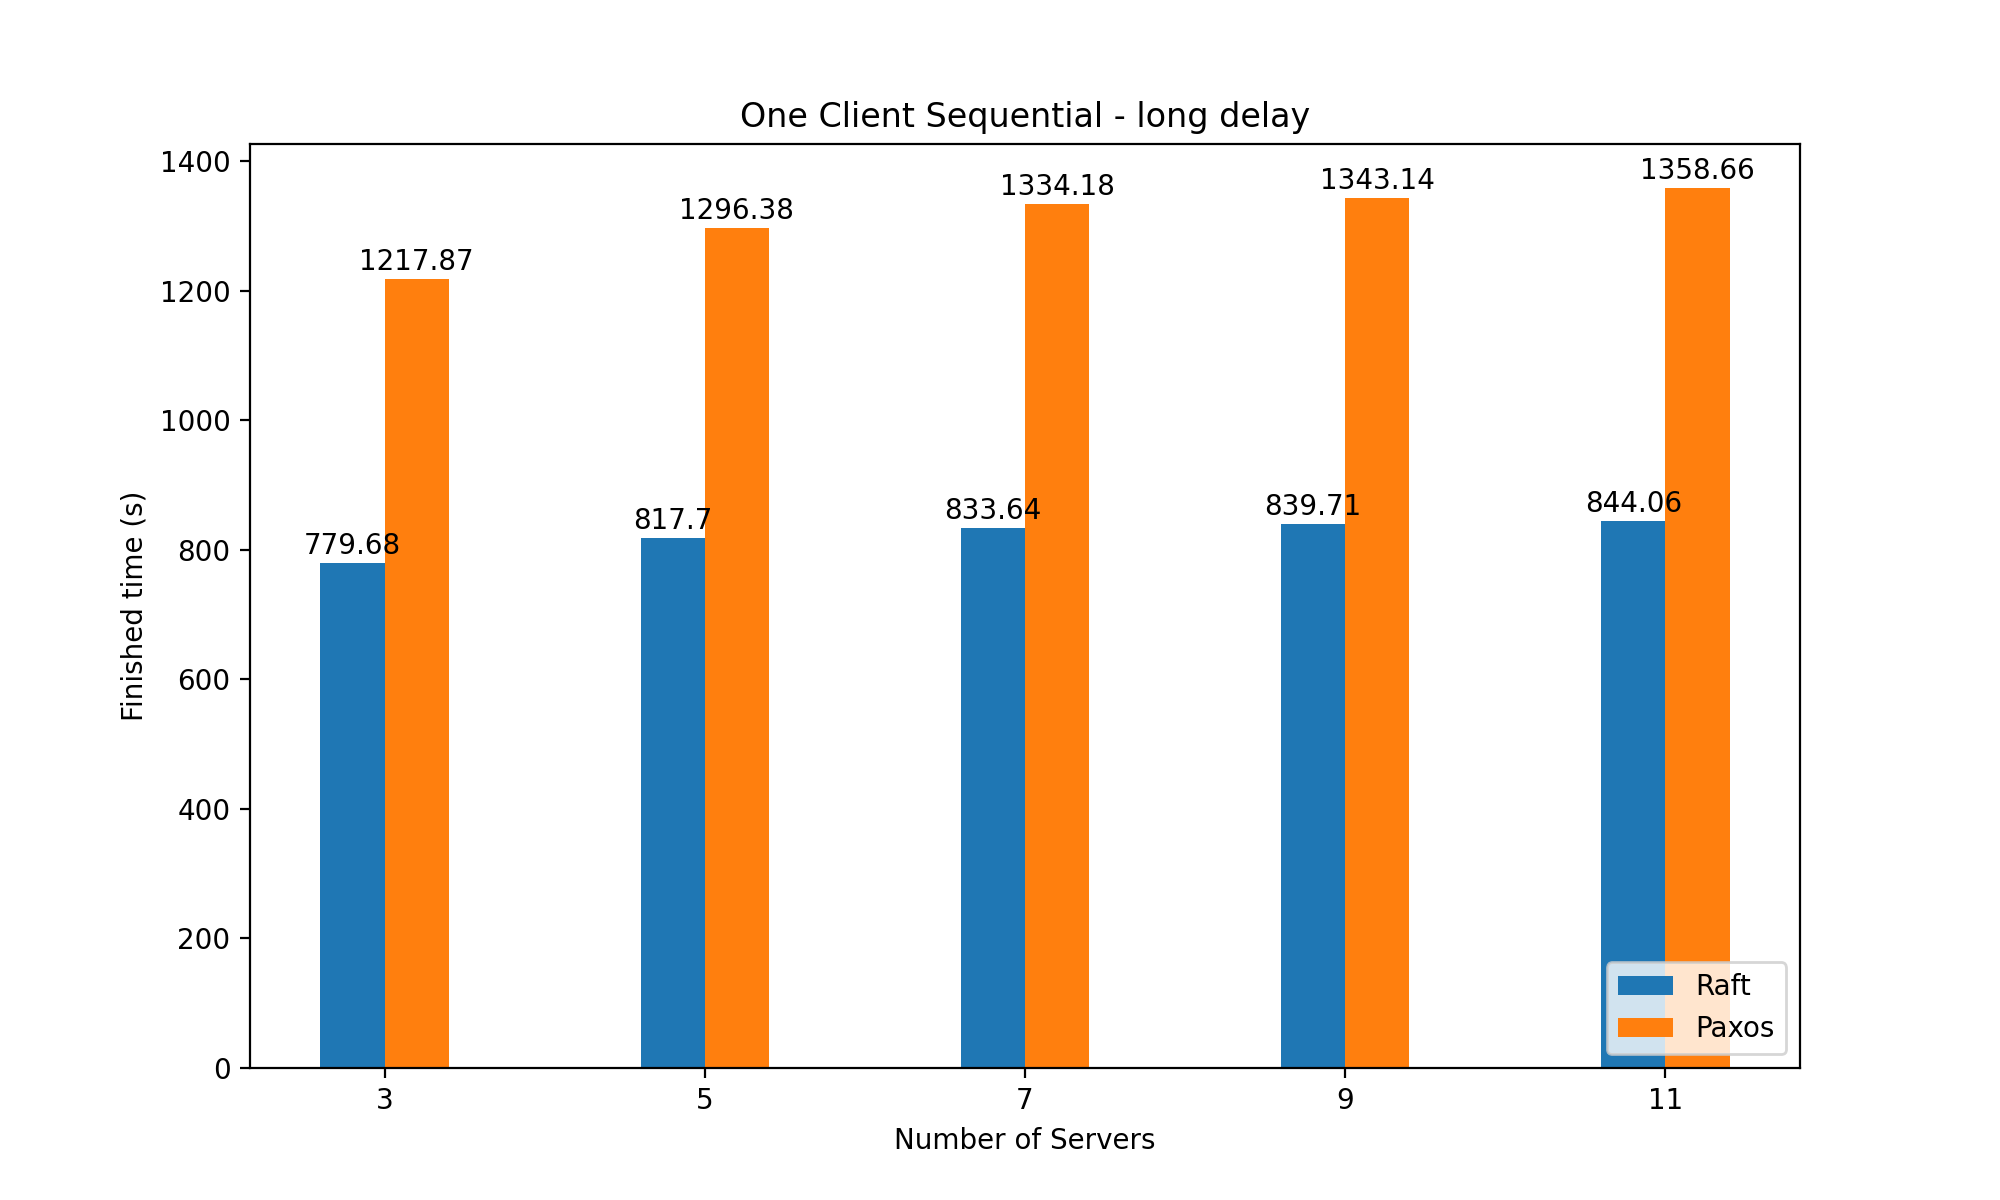
\includegraphics[width=\linewidth]{figures/one_cli_long_delay.png}
        \caption{}
    \end{subfigure}
    \hfill
    \begin{subfigure}{0.48\textwidth}
        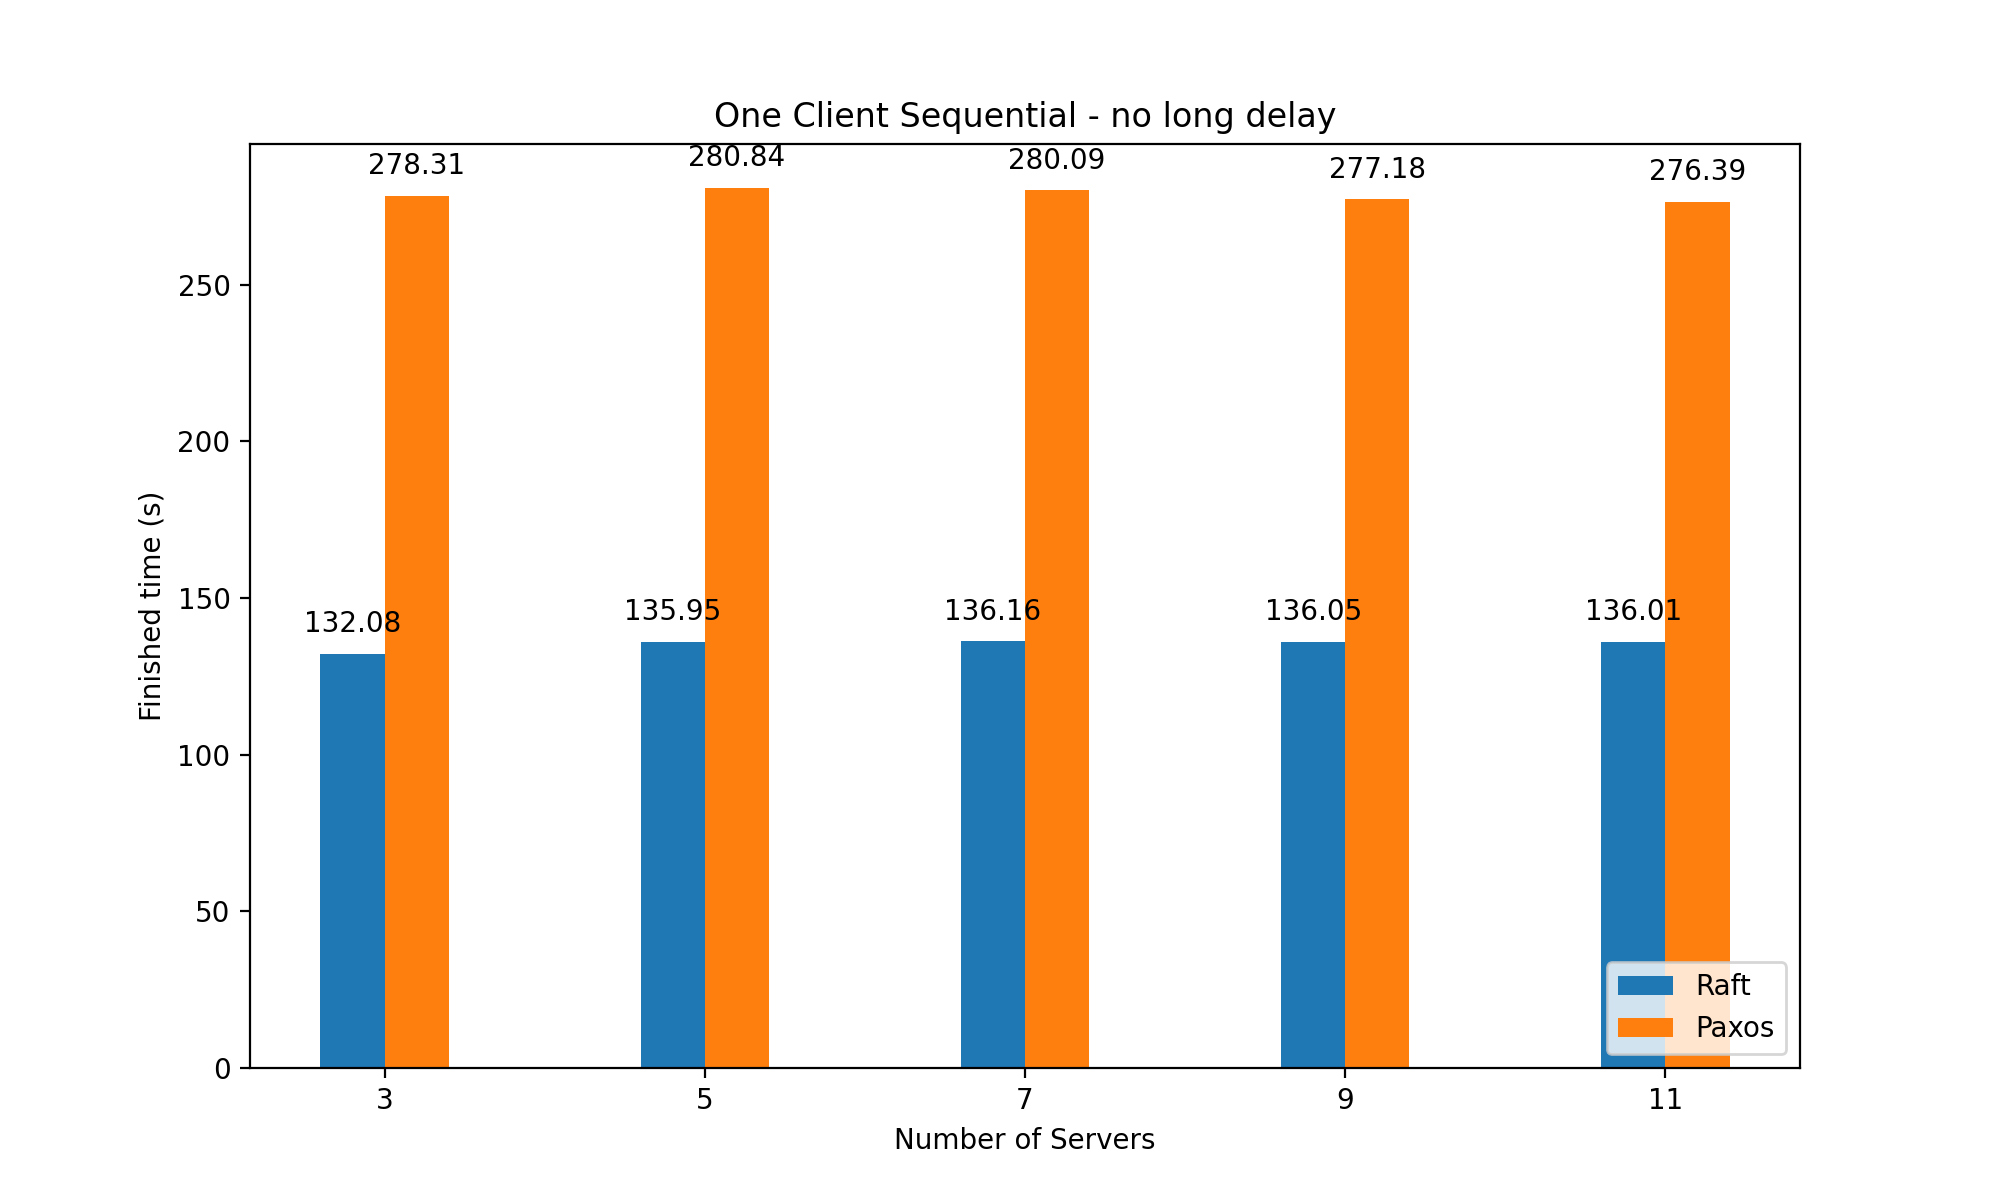
\includegraphics[width=\linewidth]{figures/one_cli_no_long_delay.png}
        \caption{}
    \end{subfigure}
    \caption{Speed test of single client: (a) with long delay network setting (b) without long delay network setting}
    \label{fig:speed_singleClient}
\end{figure}

The Raft and Paxos algorithms fundamentally incur different network overheads. Raft requires 2 RPCs (client to server, leader to follower) while Paxos requires 3 RPCs (client to server, prepare phase, and promise phase). As expected, Raft performs better with shorter finished time in both long delay and no long delay network setting (Figure \ref{fig:speed_singleClient}). Besides RPC cost, Paxos requires additional communication cost - Raft will notify servers immediately after acheiving consensus, whereas Paxos relies on servers periodically querying Paxos to check for consensus. As shown in Figure \ref{fig:speed_singleClient} (b), Raft is almost 2x faster than Paxos considering both RPC cost and additional communicate cost. However, RPC cost dominates the finished time under long delay scenario, thus Raft becomes 1.5x faster than Paxos. (Figure \ref{fig:speed_singleClient} (a))

When increasing servers number, the increasing of finished time is not apparent since the communication between servers is parallel. In long delay setting (Figure \ref{fig:speed_singleClient} (a)), finished time only increase 1.08x - 1.1x when number of servers increase from 3 to 11, showing that RPC cost is the bottleneck in this experiment.

\subsubsection{MultipleClientsParallel}

\begin{figure}[!ht]
    \begin{subfigure}{0.48\textwidth}
        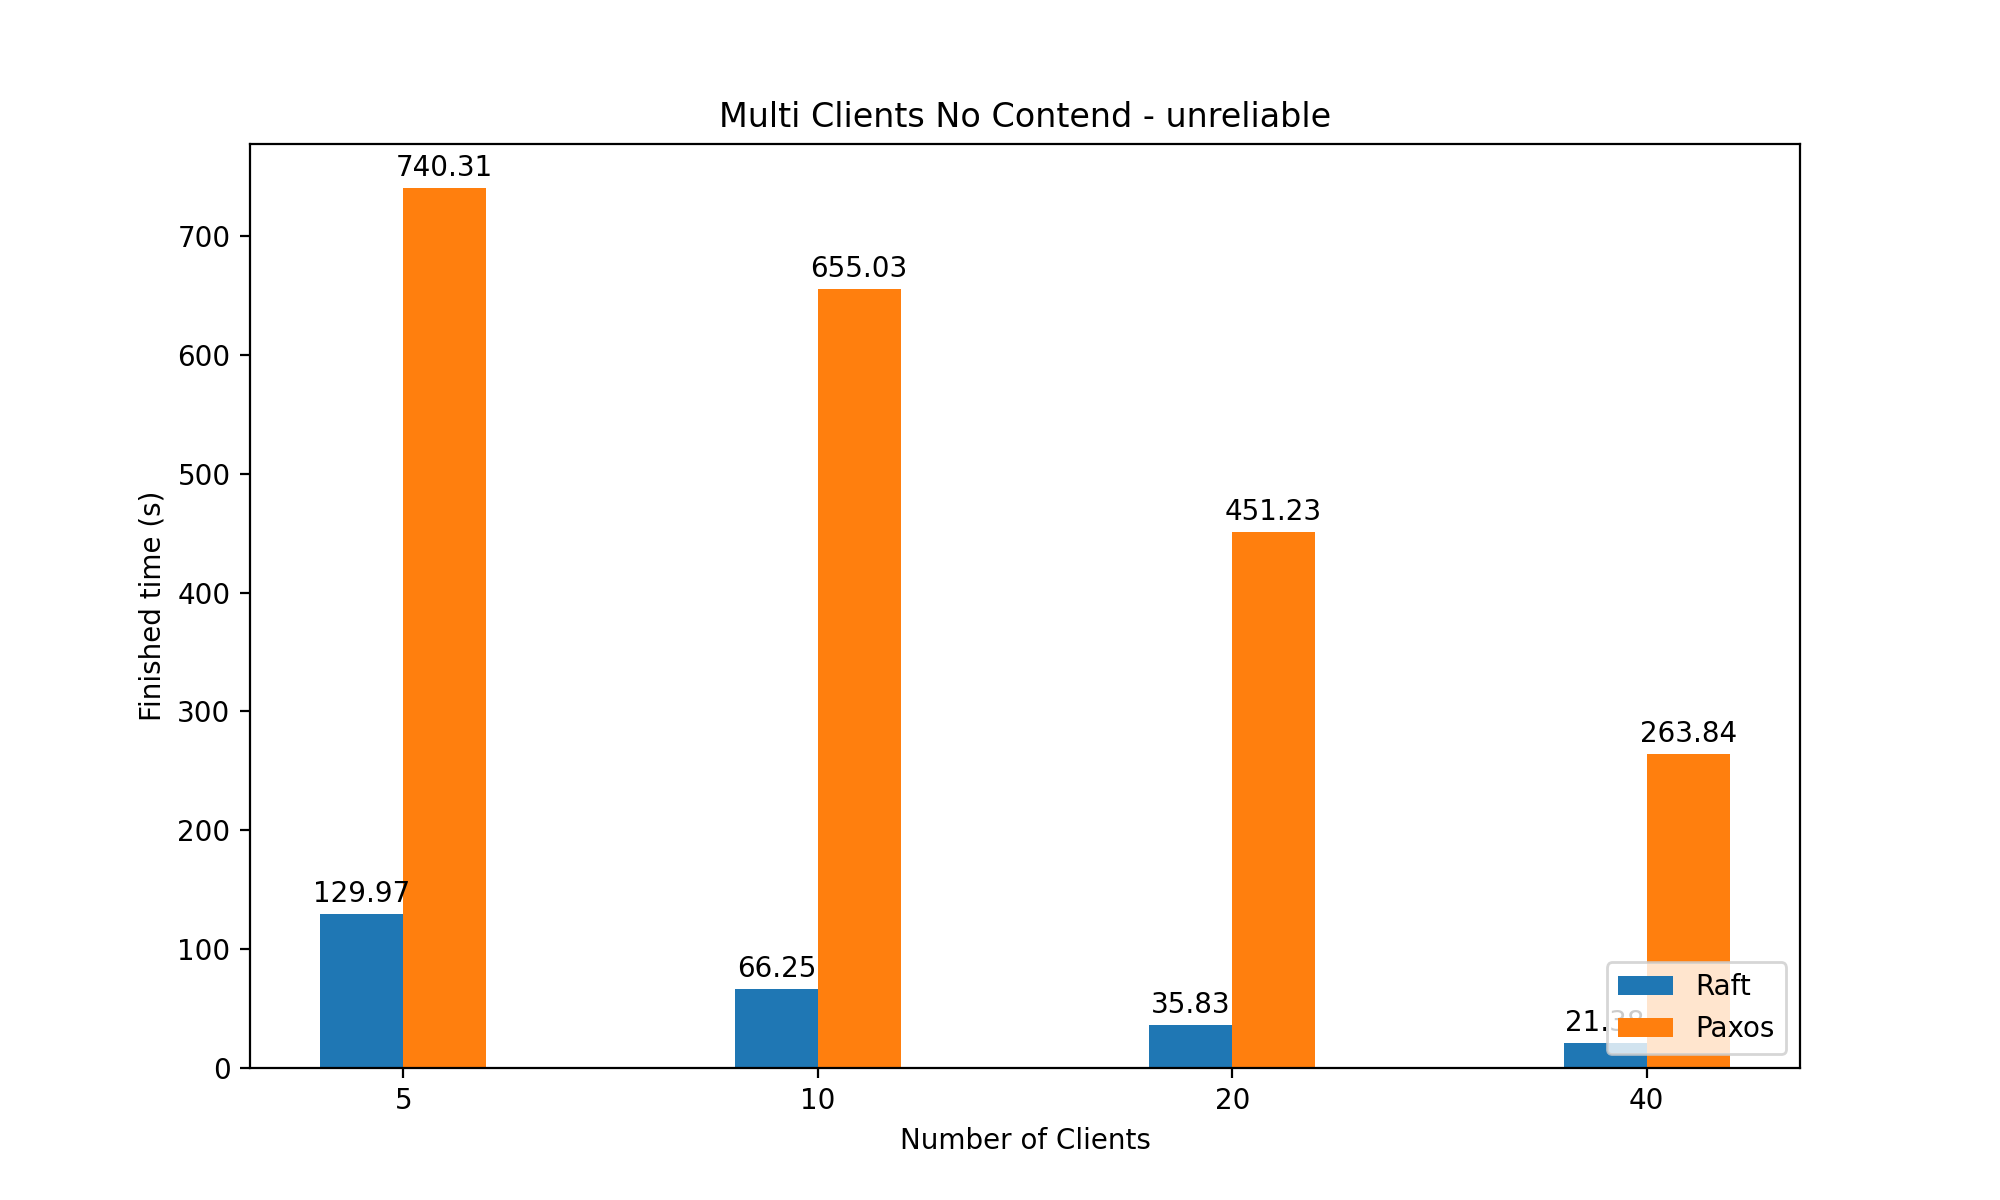
\includegraphics[width=\linewidth]{figures/multi_cli_no_contend_no_unreliable.png}
        \caption{}
    \end{subfigure}
    \hfill
    \begin{subfigure}{0.48\textwidth}
        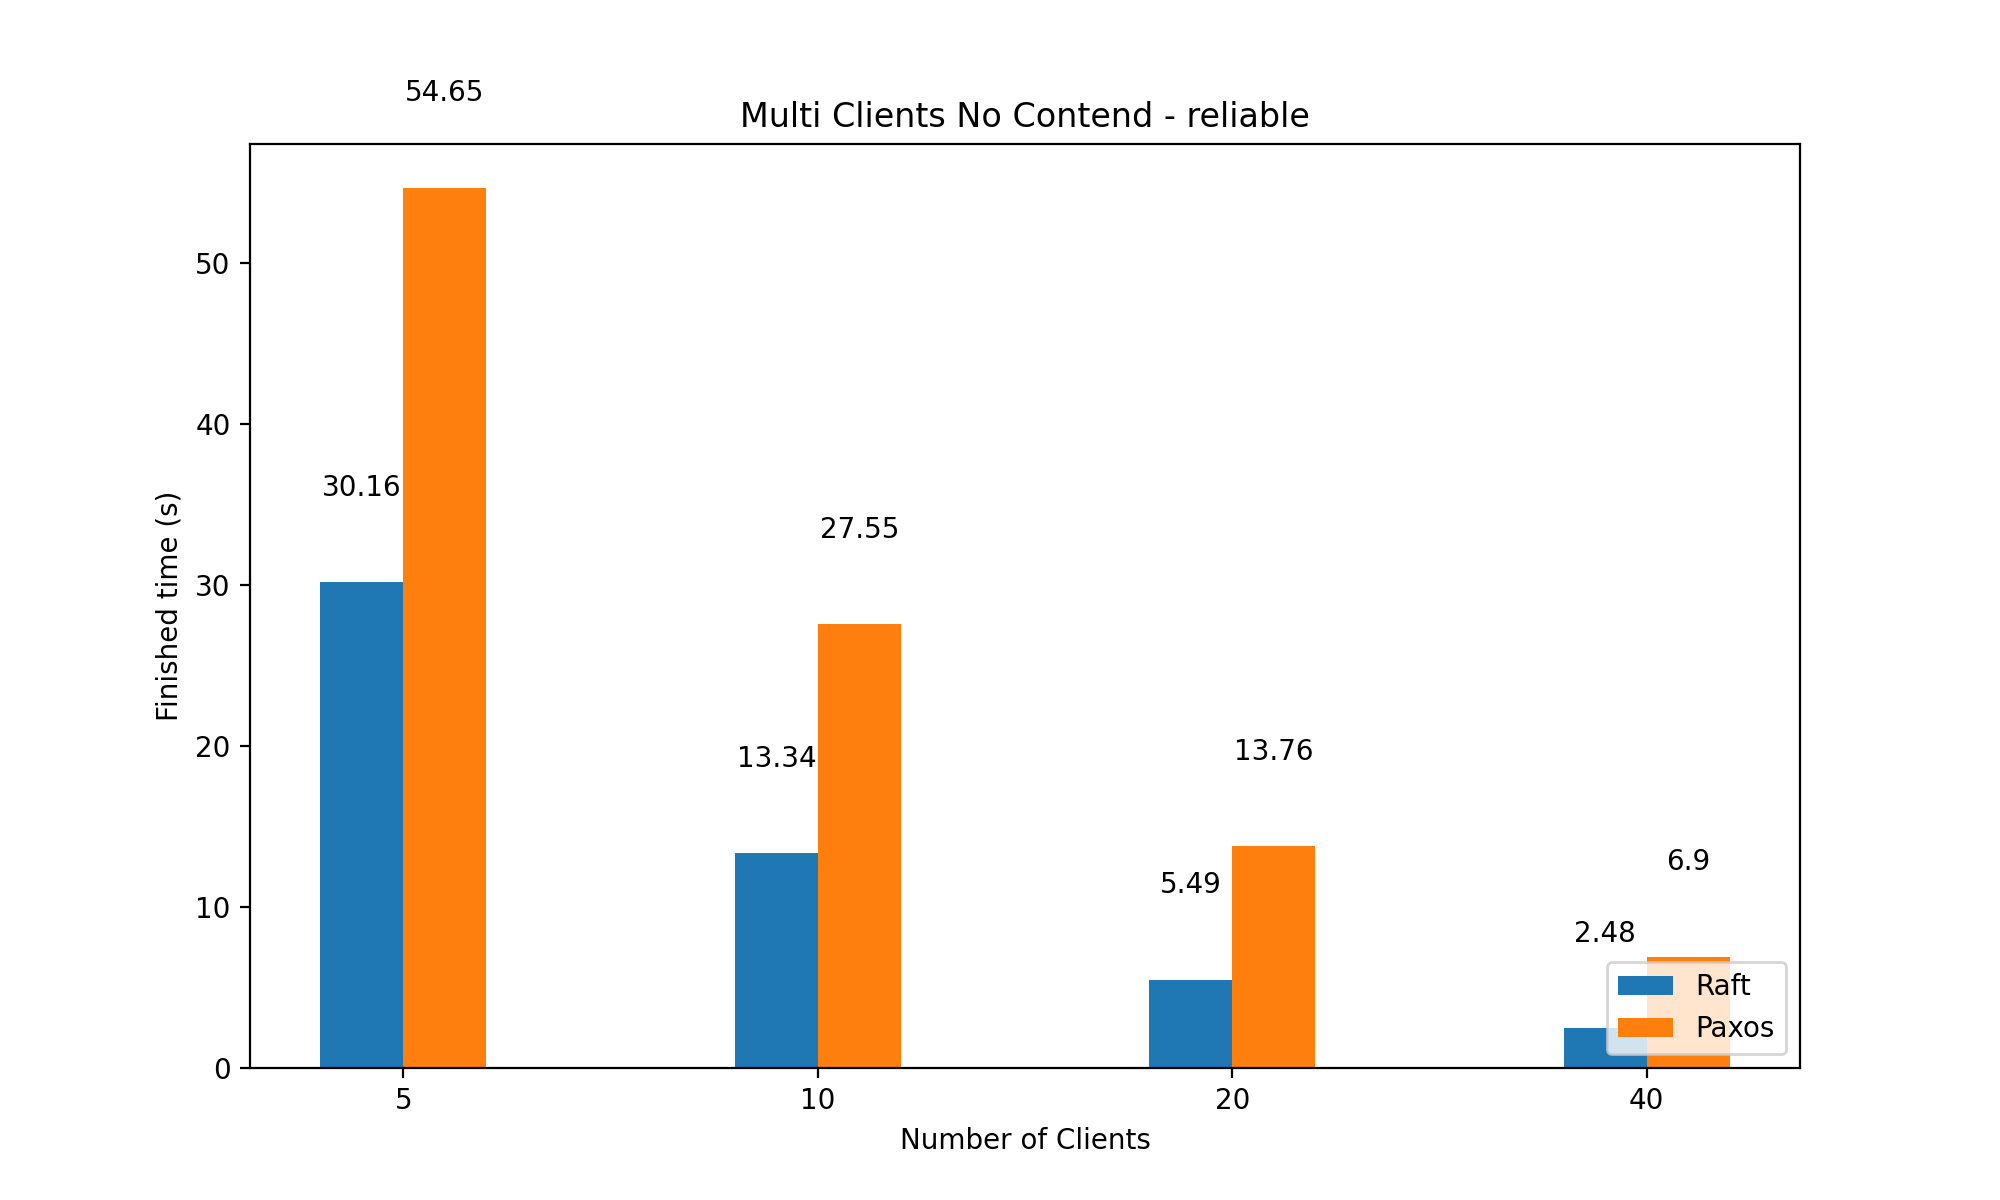
\includegraphics[width=\linewidth]{figures/multi_cli_no_contend_reliable.png}
        \caption{}
    \end{subfigure}
    \caption{Speed test of multiple clients parallel: (a) with unreliable network setting (b) with reliable network setting}
    \label{fig:speed_MultipleClientsParallel}
\end{figure}

In MultipleClientsParallel experiment, as expected, the termination time decrease as the number of clients increase since both Raft and Paxos servers can handle multiple client requests simultaneously. As shown in Figure \ref{fig:speed_MultipleClientsParallel}, when number of clients doubles, the completion time also half. Moreover, Raft performs better than Paxos as predicted due to their algorithm design.

In our implementation, since Raft can batch multiple requests in a single RPC call, it shows more noticeable improvement as the number of clients grows. Raft's performance increases by 12x, whereas Paxos only improves by 8x when the number of clients increases by 8x (Figure \ref{fig:speed_MultipleClientsParallel} (b)).

Interestingly, unreliable network setting has a greater impact on Paxos - when there are only five clients, the completion time of Paxos increases by 13.7 times, while Raft only increases by 4.3 times (Figure \ref{fig:speed_MultipleClientsParallel} (a)). We believe this is because Paxos requires individual resolutions for each request, and any dropped requests during the prepare, promise, or accept phases could potentially result in the failure of the consensus.

\subsubsection{MultipleClientsContention}

\begin{figure}[!ht]
\centering
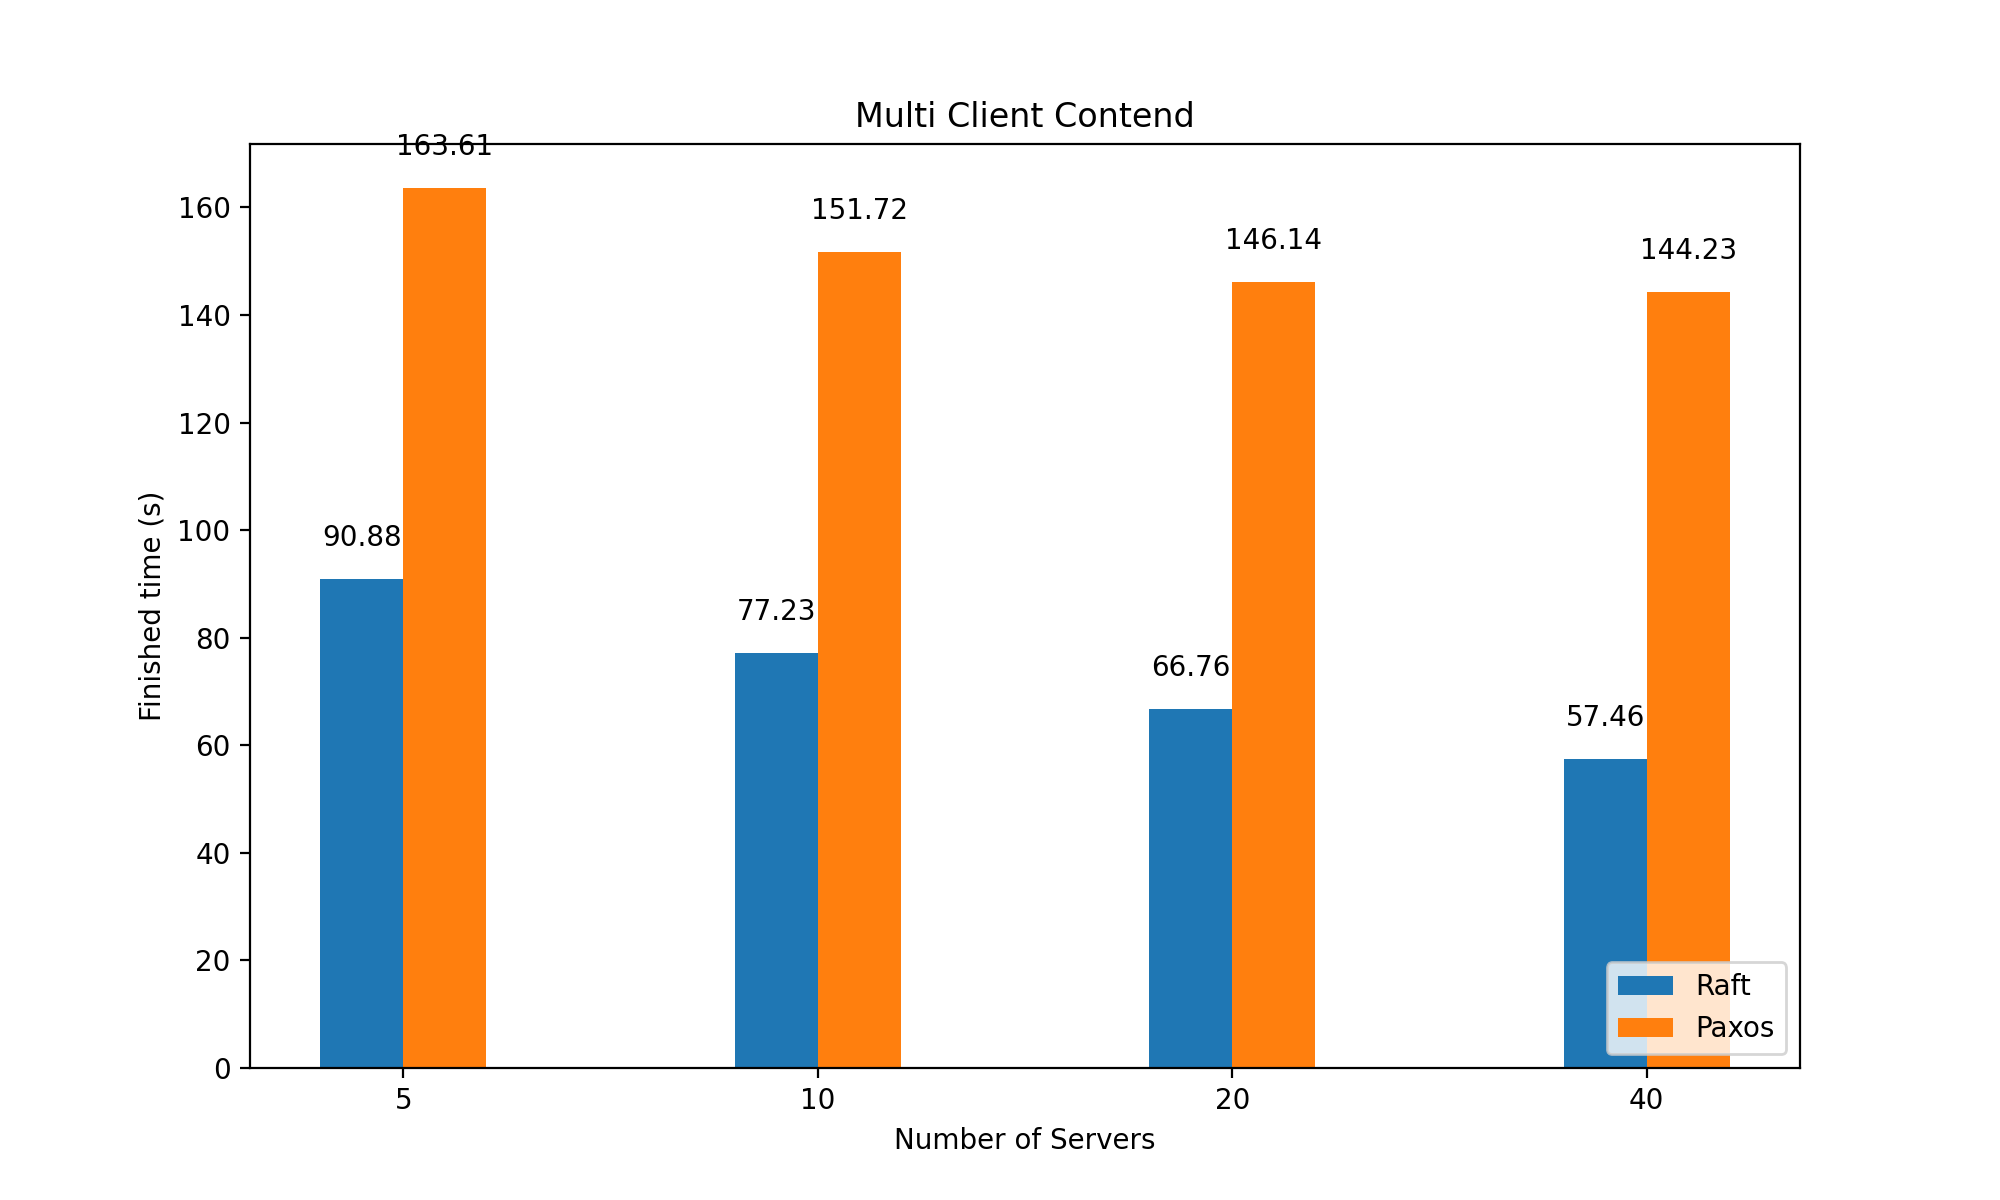
\includegraphics[width=0.5\linewidth]{figures/multi_cli_contend.png}
\caption{\label{fig:speed_MultipleClientsContention}Speed test of multiple clients contention}
\end{figure}

Under conditions of client contention, augmenting the client count yields marginal enhancements in performance. Comparing Figure \ref{fig:speed_MultipleClientsParallel} (b) and \ref{fig:speed_MultipleClientsContention}, it is evident that under non-contention conditions, the throughput of Raft and Paxos increases by factors of 13.7 and 4.3, respectively, when the number of clients is multiplied by eight. However, under contention circumstances, Raft and Paxos only experience modest improvements of 1.58 and 1.13, respectively. This is because the only area where performance can be enhanced as the number of clients increases is when a release request coincides with an incoming acquire request, allowing the acquire request to be promptly fulfilled.

\subsection{Failure Test}
\subsubsection{MultipleClientsParallel with LeaderFailure}

\begin{figure}[!ht]
    \begin{subfigure}{0.49\textwidth}
        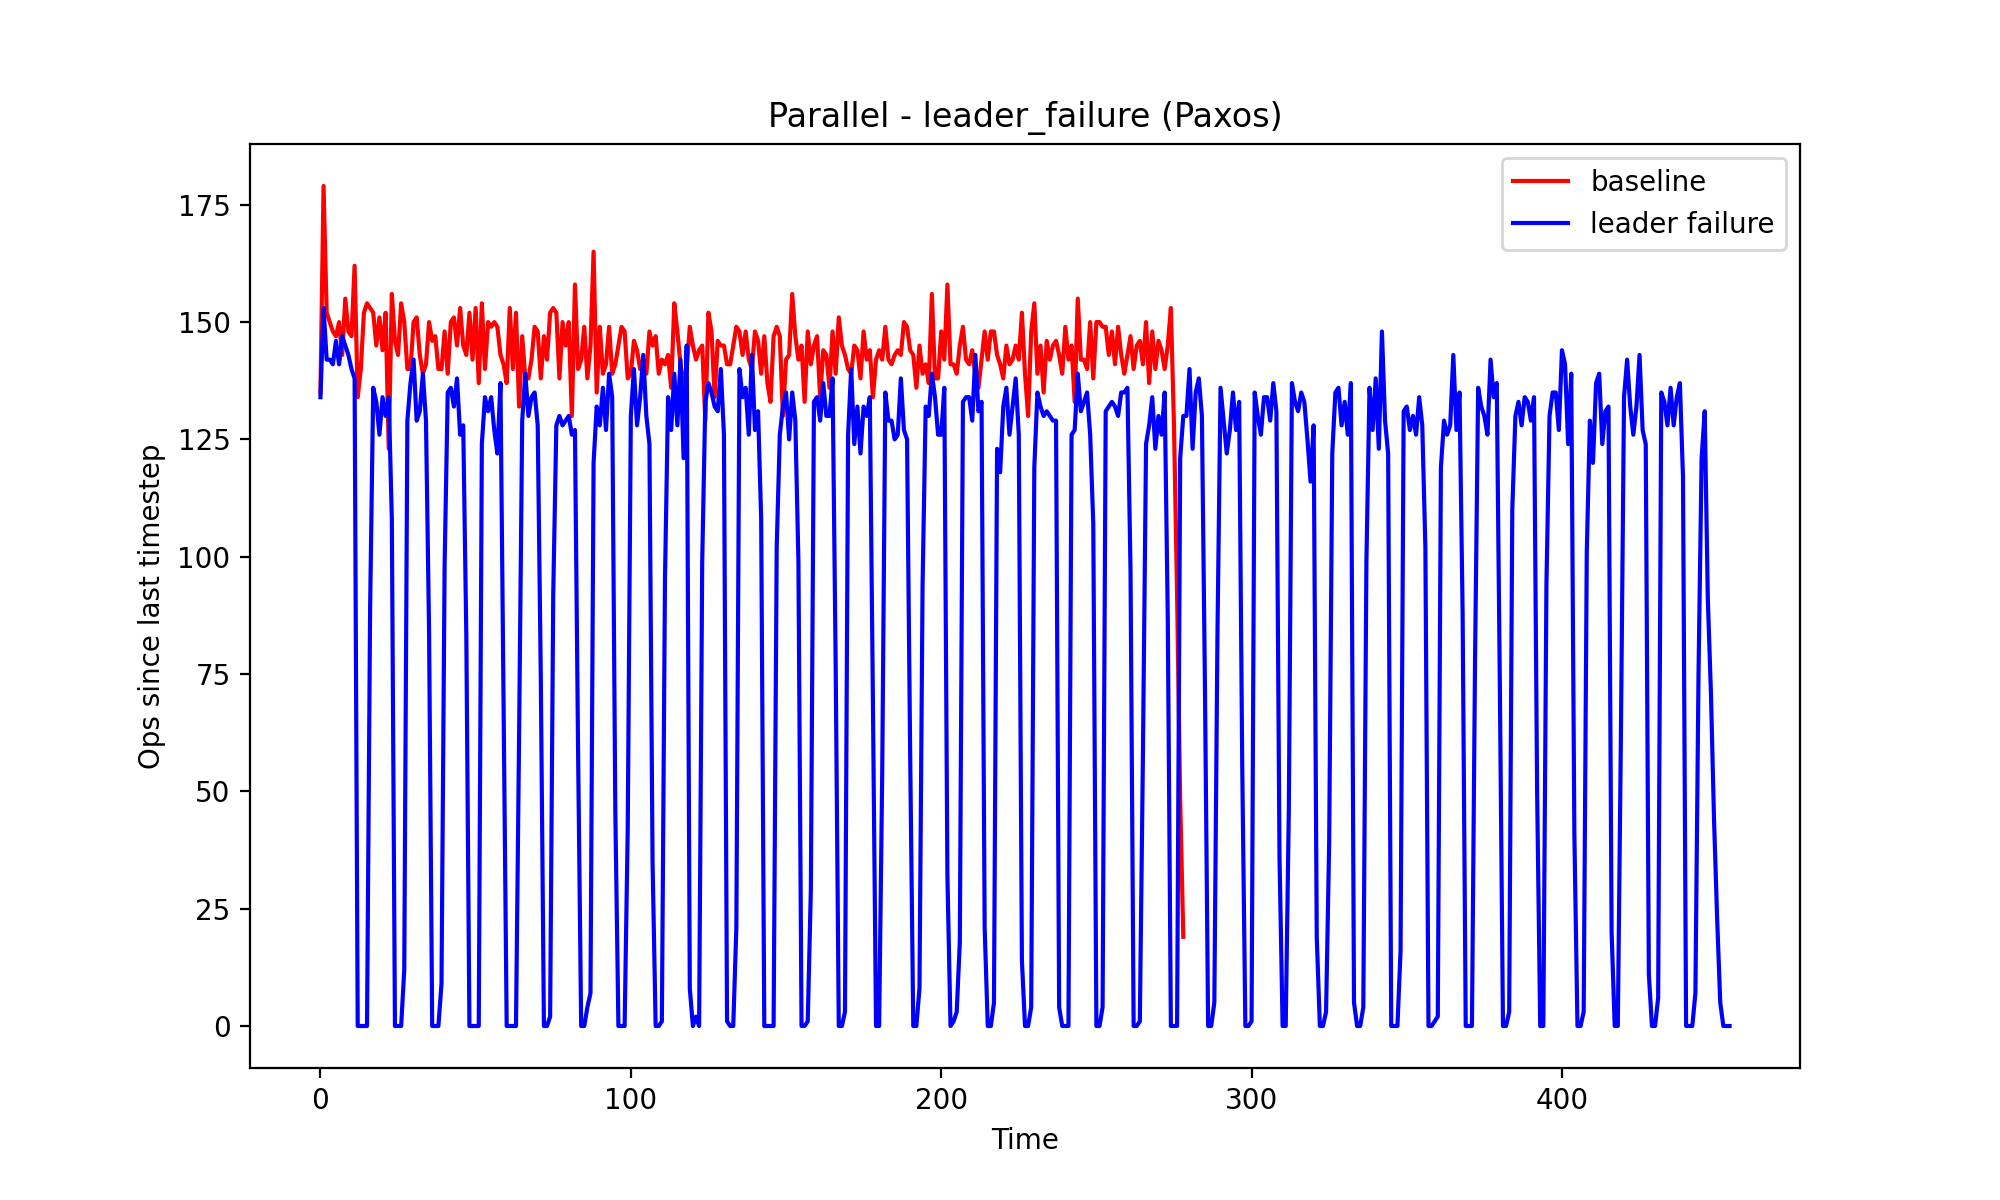
\includegraphics[width=\linewidth]{figures/para-lf-Paxos.png}
        \caption{}
    \end{subfigure}
    \begin{subfigure}{0.49\textwidth}
        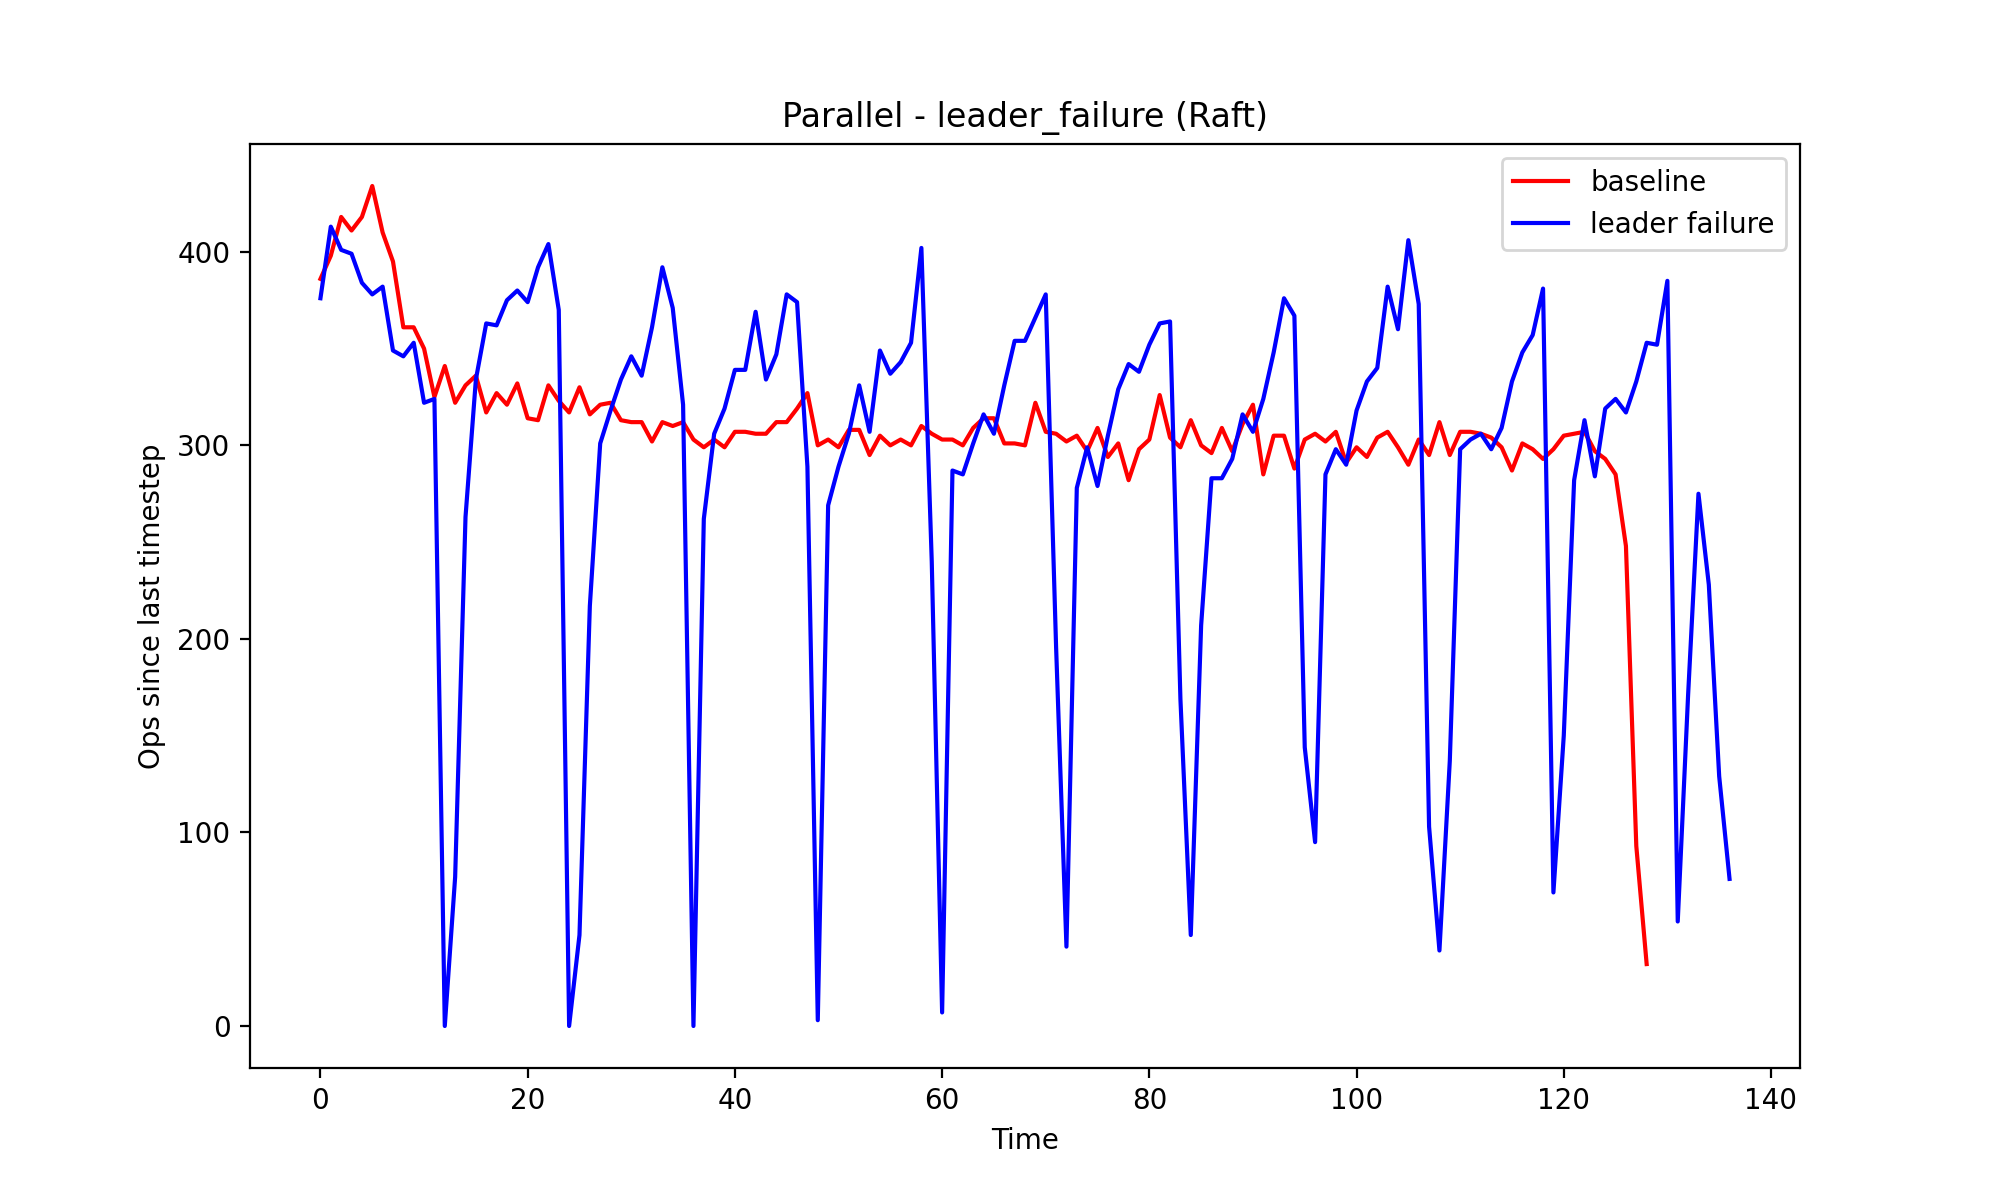
\includegraphics[width=\linewidth]{figures/para-lf-Raft.png}
        \caption{}
    \end{subfigure}
    \caption{Failure test of leader failure with multiple clients parallel: (a) Paxos (b) Raft}
    \label{fig:failure_LeaderFailure_MultipleClientsParallel}
\end{figure}

Experimental findings demonstrate that even in the event of leader failure, our system continues to operate smoothly. As depicted in the Figure \ref{fig:failure_LeaderFailure_MultipleClientsParallel}, for every 12 seconds, operations are required to await the election of a new leader before proceeding.

As discussed earlier, Raft's performance tends to surpass that of Paxos. Analysis of the experimental results reveals that in the event of leader failure, Paxos experiences an approximately 1.5-fold delay before completion, whereas Raft encounters only around a 1.01-fold delay.

Furthermore, we have observed an intriguing phenomenon: upon the generation of a new leader, the operational throughput in Raft momentarily surpasses the baseline throughput. This can be attributed to the process of leader failure, where although some operations remain incomplete, they have already been partially synchronized with some servers. Consequently, upon the emergence of a new leader, completing these half-way operations becomes faster.

\subsubsection{MultipleClientsContention with LeaderFailure}

\begin{figure}[!ht]
    \begin{subfigure}{0.49\textwidth}
        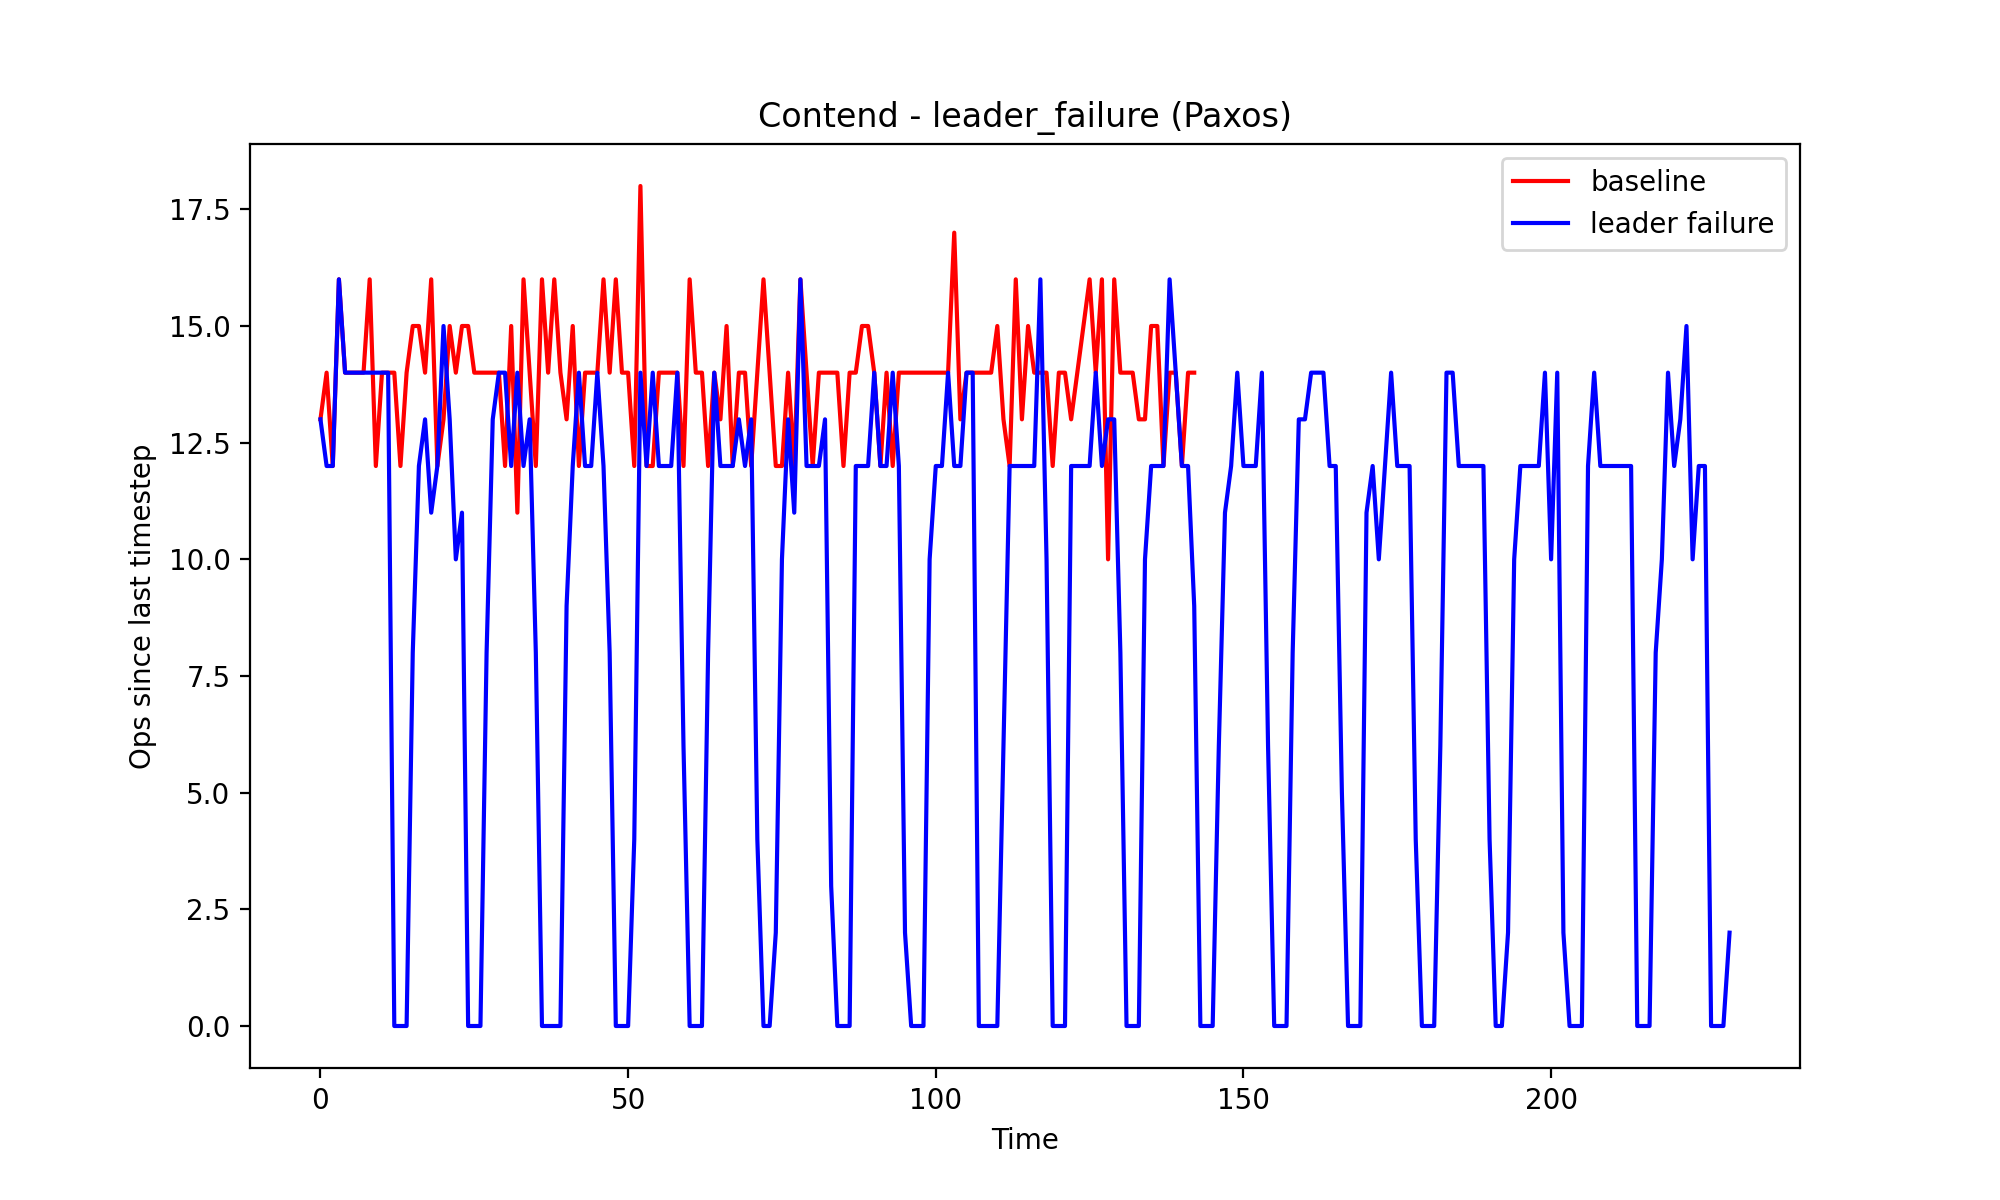
\includegraphics[width=\linewidth]{figures/cont-lf-Paxos.png}
        \caption{}
    \end{subfigure}
    \begin{subfigure}{0.49\textwidth}
        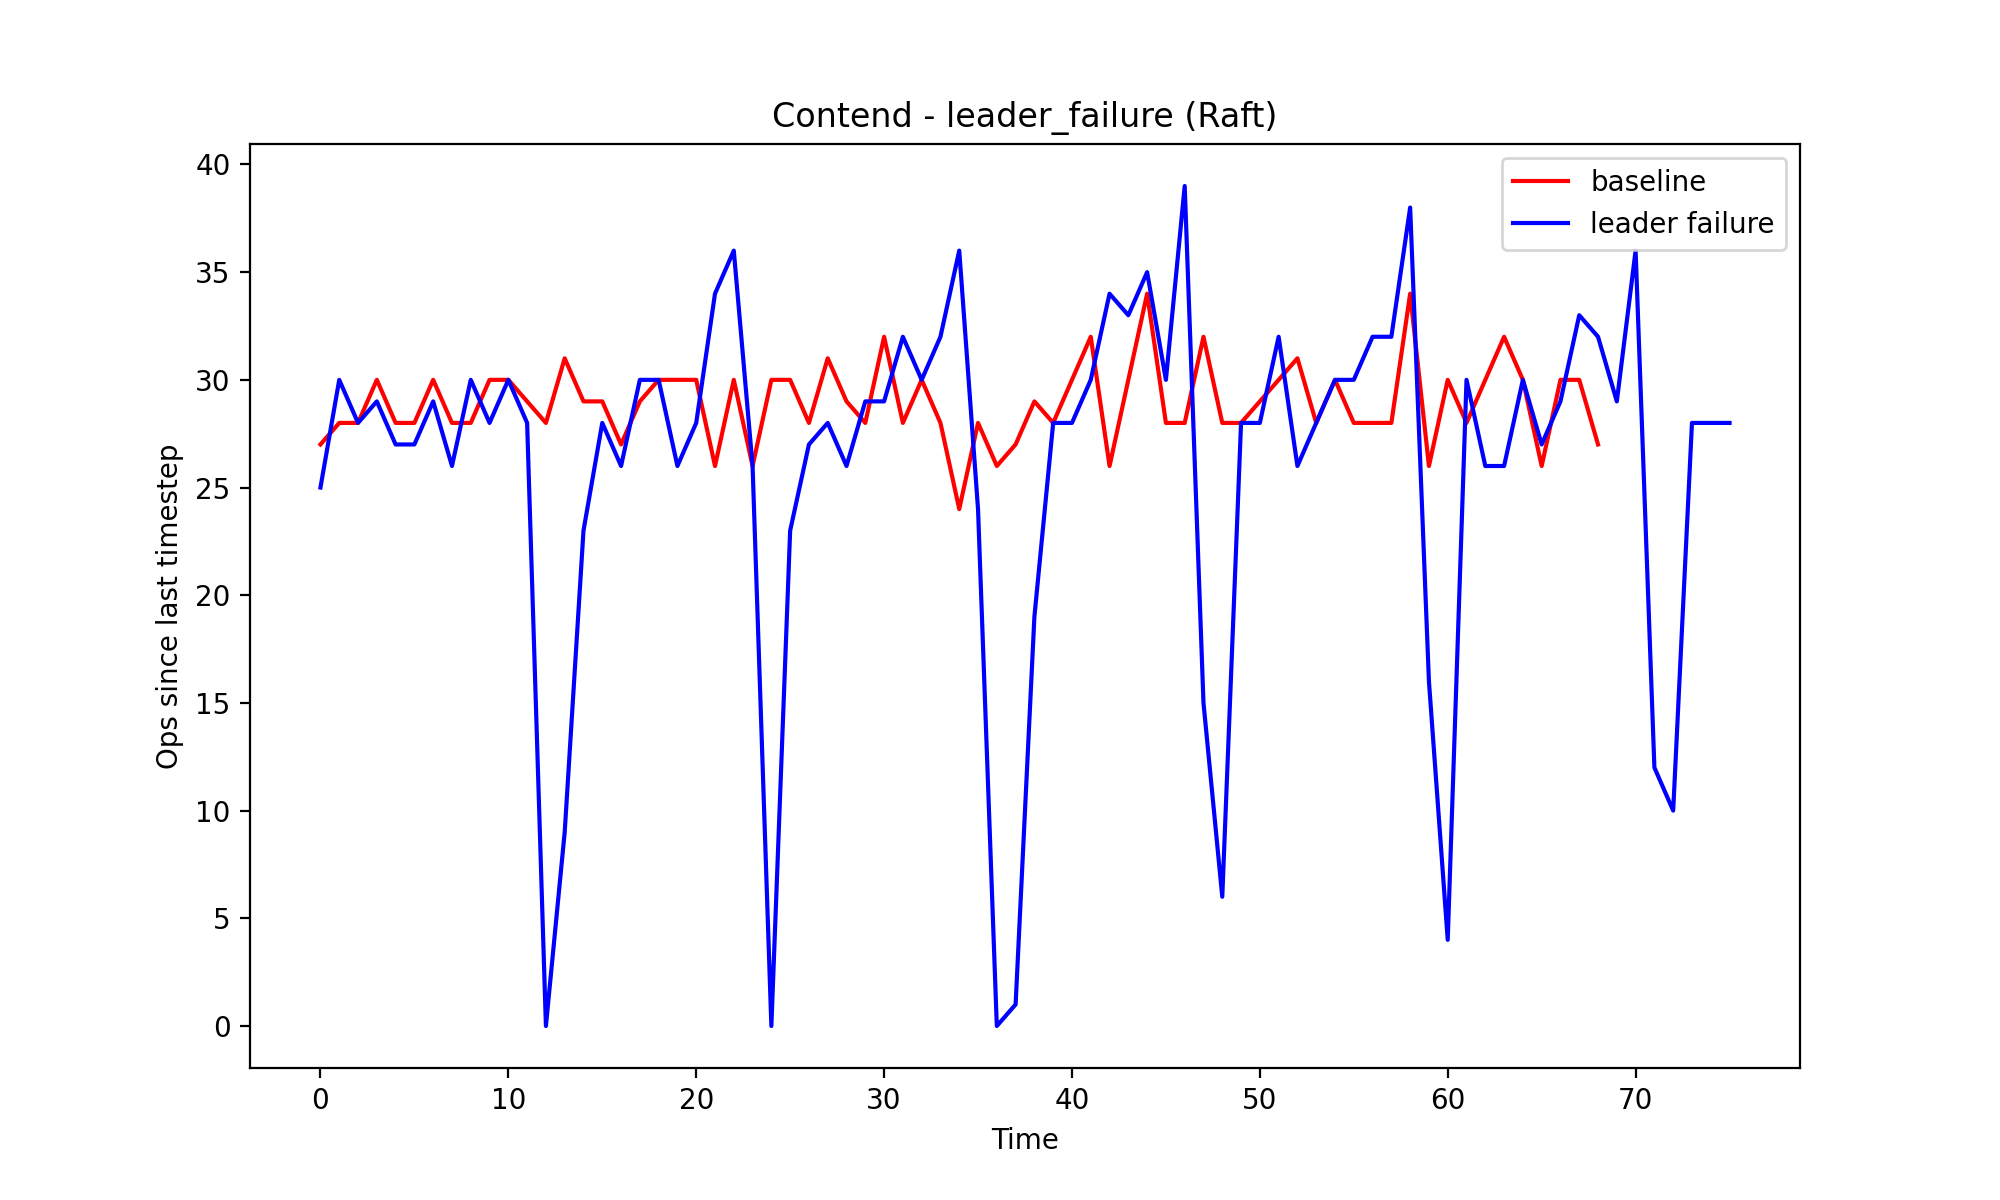
\includegraphics[width=\linewidth]{figures/cont-lf-Raft.png}
        \caption{}
    \end{subfigure}
    \caption{Failure test of leader failure with multiple clients contention: (a) Paxos (b) Raft}
    \label{fig:failure_LeaderFailure_MultipleClientsContention}
\end{figure}

Our system ensures that even in the scenario of multiple clients competing for the same lock and a leader failure, system functionality remains operational. In this scenario, as expected, Raft's performance still surpasses Paxos (Figure \ref{fig:failure_LeaderFailure_MultipleClientsContention}). Additionally, it can be observed that Paxos requires more time to recover after failure. The reason is that Paxos, in order to ensure the sequence of operations, must ensure that all preceding operations are decided before proceeding with new operations. Each preceding operation is independent and has its own waiting time. However, after electing a new leader, Raft will have the new leader batch all operations that occurred during the failure period and synchronously distribute them to all followers at once.

\subsubsection{MultipleClientsParallel with NonLeaderFailure}

\begin{figure}[!ht]
    \begin{subfigure}{0.49\textwidth}
        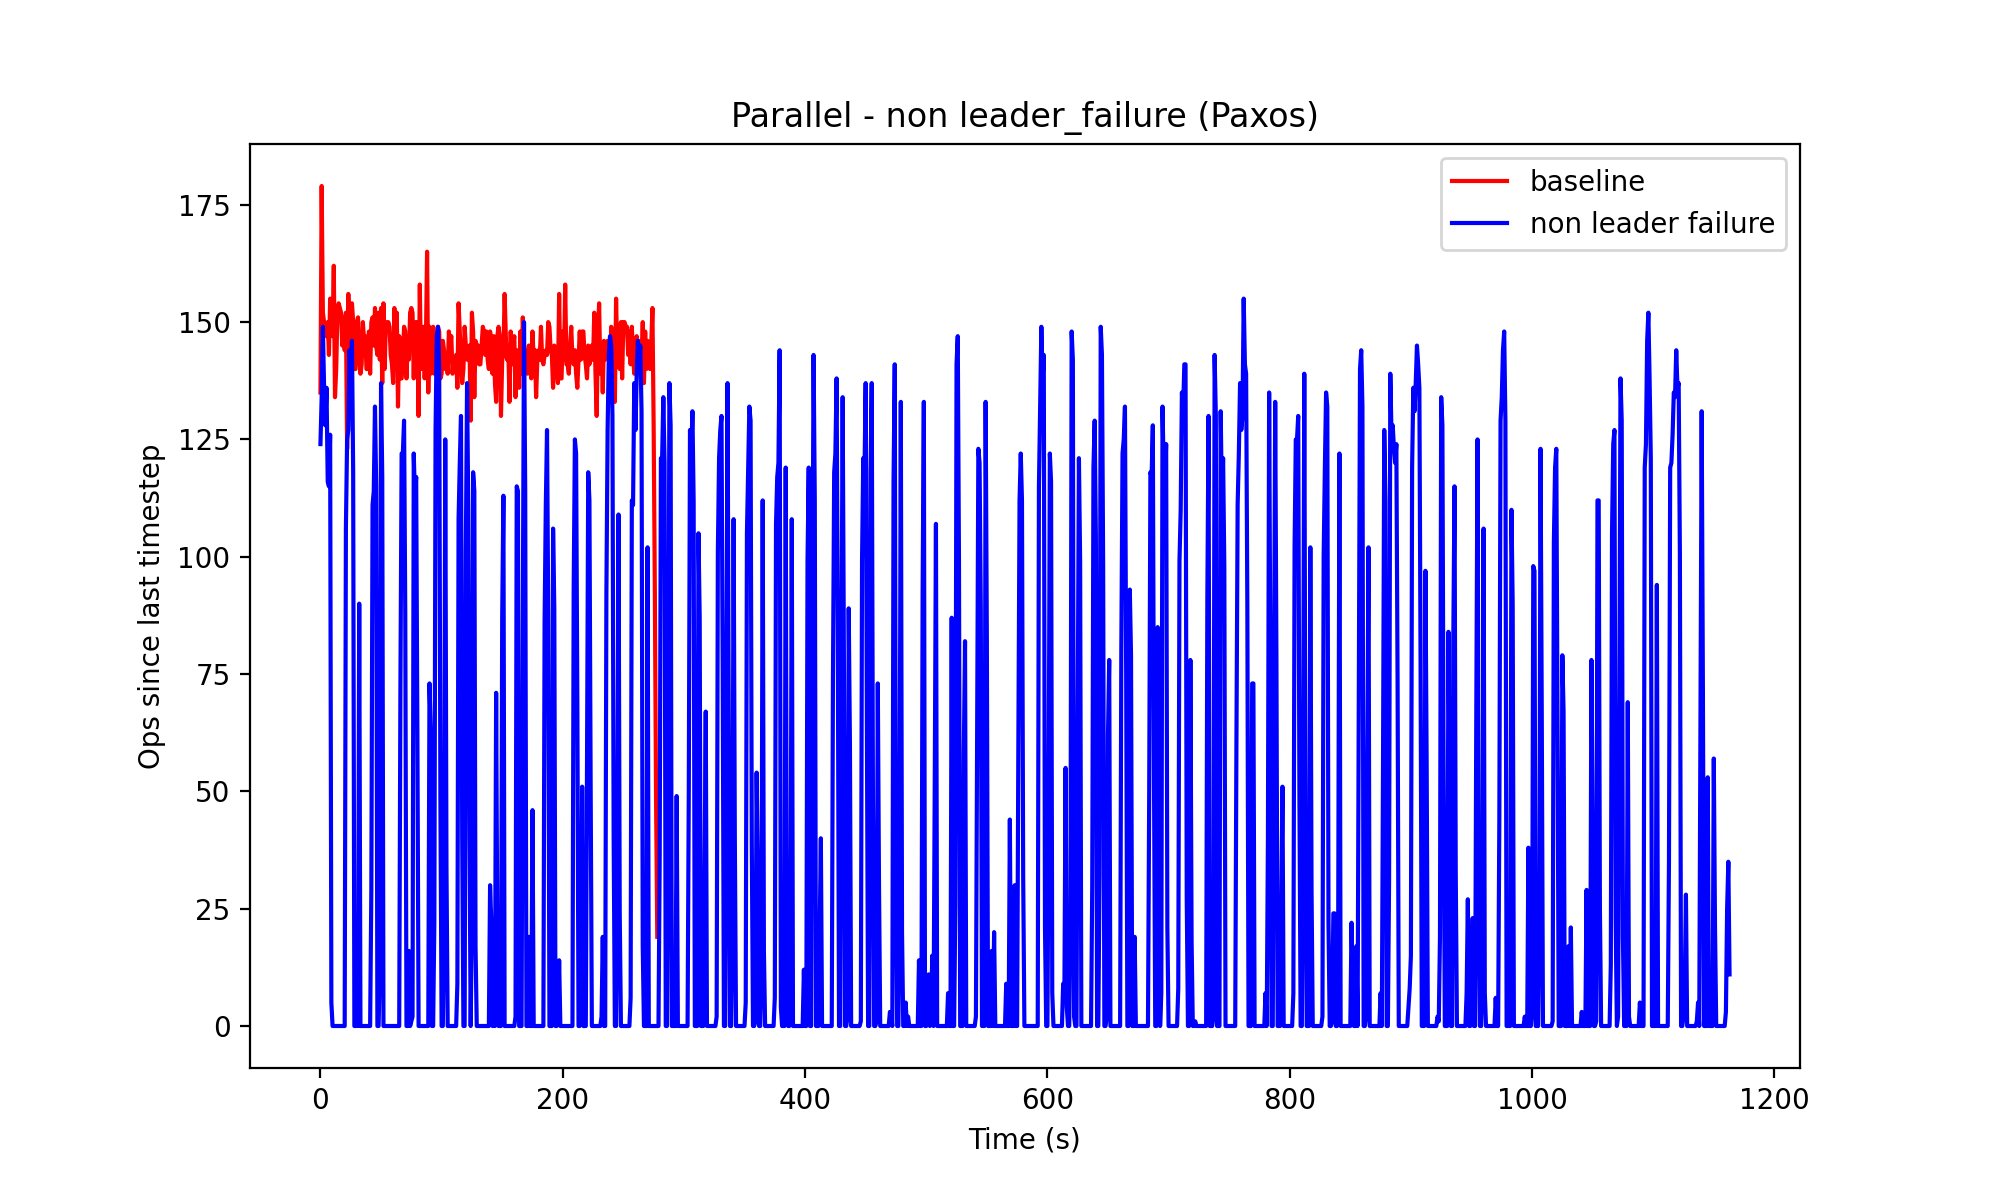
\includegraphics[width=\linewidth]{figures/para-nlf-Paxos.png}
        \caption{}
    \end{subfigure}
    \begin{subfigure}{0.49\textwidth}
        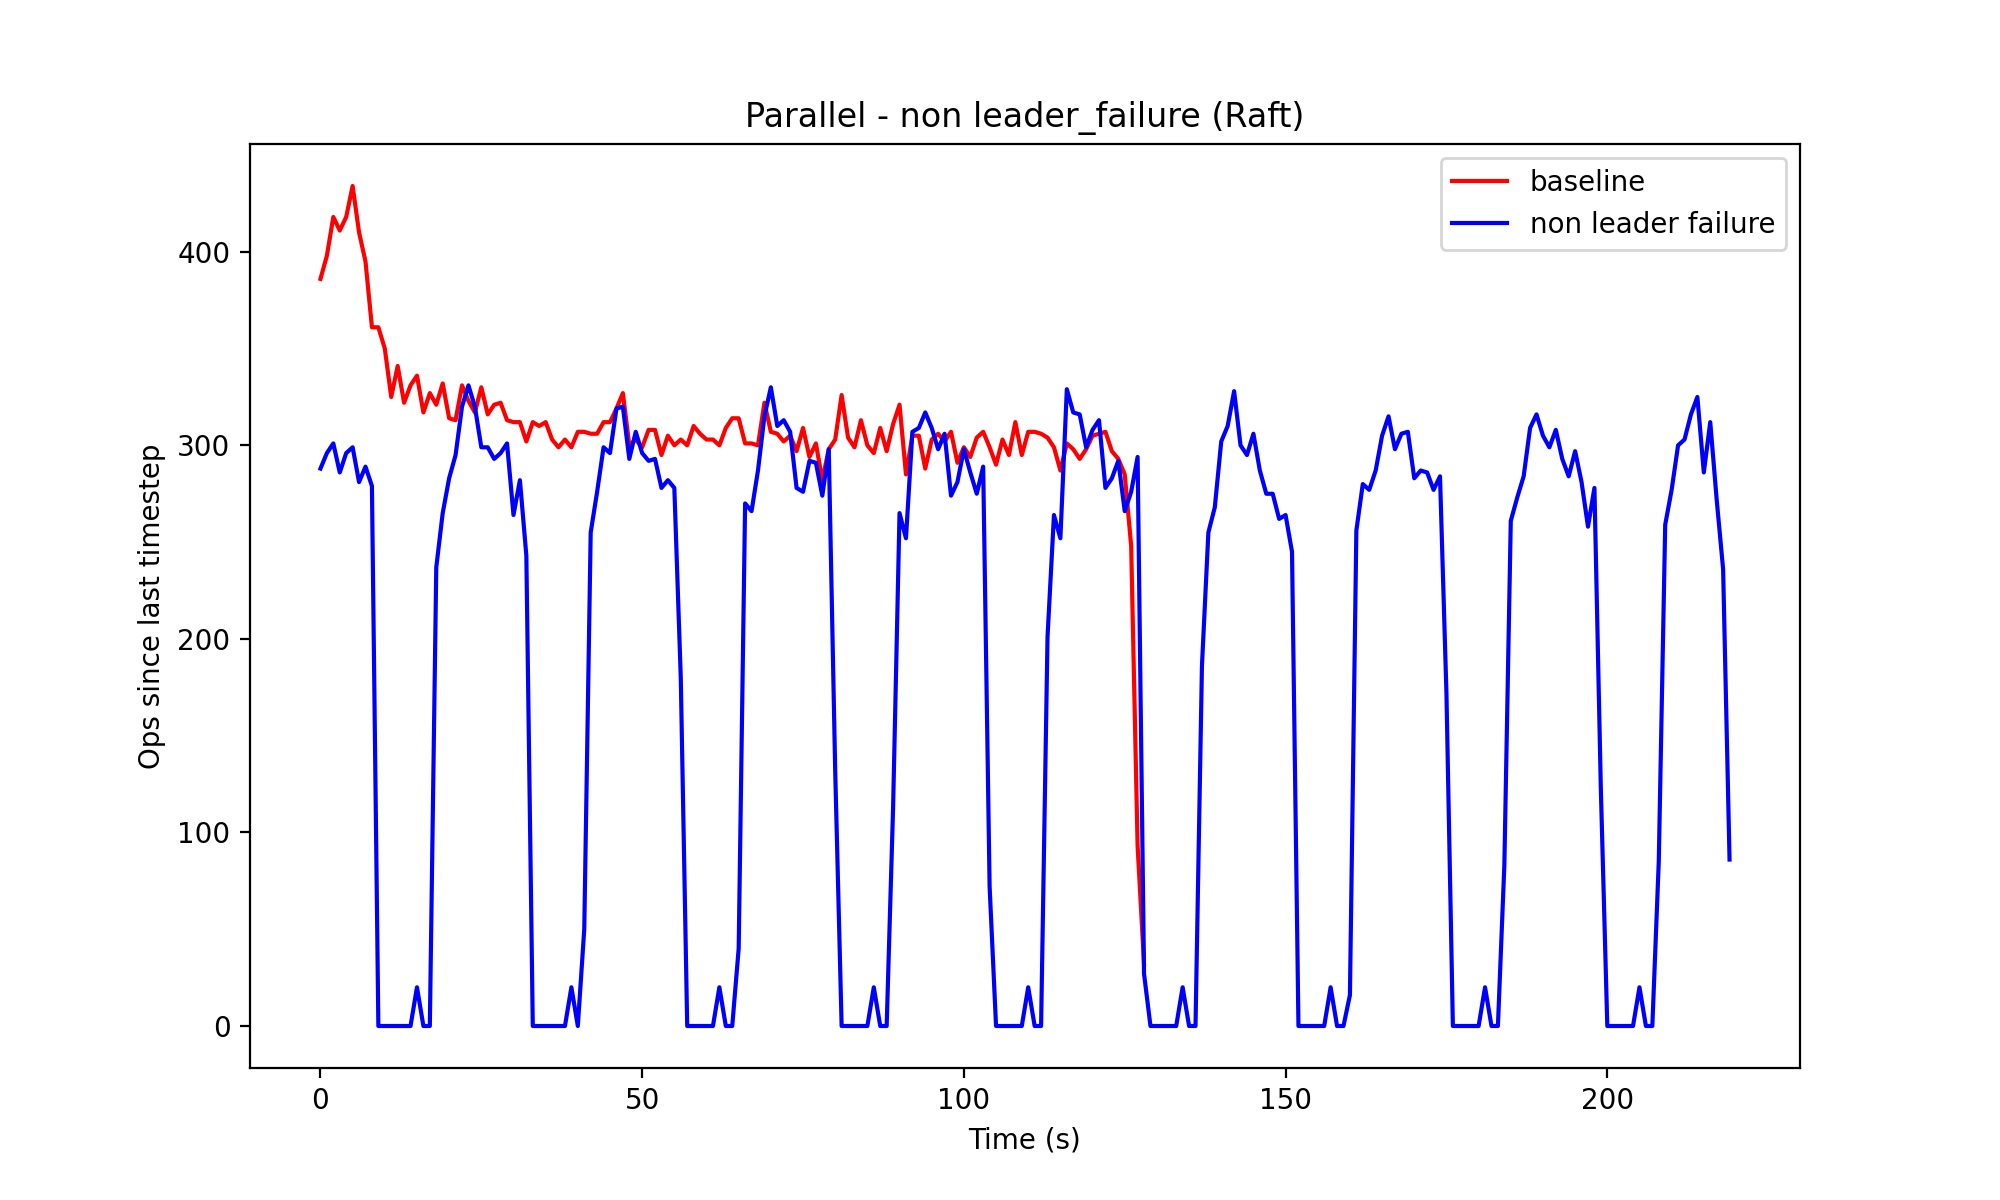
\includegraphics[width=\linewidth]{figures/para-nlf-Raft.png}
        \caption{}
    \end{subfigure}
    \caption{Failure test of non leader failure with multiple clients parallel: (a) Paxos (b) Raft}
    \label{fig:failure_NonLeaderFailure_MultipleClientsParallel}
\end{figure}

This experiment sheds light on the role of 'majority vote' in consensus algorithms. From Figure \ref{fig:failure_NonLeaderFailure_MultipleClientsParallel} (b), it can be observed that when 3 or 4 servers are down, due to the inability to achieve a majority, operations cannot proceed. It's interesting to note that when only two servers are operational, a small peak occurs. This is possibly because some operations were synchronized with the some servers that have now failed, but a majority was not reached at that time. When the second server restarts and achieves the majority, the operations can proceed. For example, consider a scenario with five servers, where only the leader and server 4 are alive. After server 4 goes down and server 1 restarts, operations that have already synchronized with server 4 will synchronize with server 1 and achieve a majority.

Another interesting phenomenon is that when only three servers are operational, the operation rate is slightly lower than the baseline. We hypothesize that this is because the baseline only needs to wait for responses from the fastest two servers to decide. However, when there are only three servers, the two servers other than the leader may be the slowest among all servers.


% Equations in \LaTeX{} can either be inline or set as display equations. For
% inline equations use the \verb+$...$+ commands. Eg: the equation
% $H\psi = E \psi$ is written via the command \verb+$H \psi = E \psi$+.

% For display equations (with auto generated equation numbers)
% one can use the equation or eqnarray environments:
% \begin{equation}
% \|\tilde{X}(k)\|^2 \leq\frac{\sum\limits_{i=1}^{p}\left\|\tilde{Y}_i(k)\right\|^2+\sum\limits_{j=1}^{q}\left\|\tilde{Z}_j(k)\right\|^2 }{p+q},
% \label{eq1}
% \end{equation}
% where
% \begin{align}
% D_\mu &=  \partial_\mu - ig \frac{\lambda^a}{2} A^a_\mu \nonumber \\
% F^a_{\mu\nu} &= \partial_\mu A^a_\nu - \partial_\nu A^a_\mu + g f^{abc} A^b_\mu A^a_\nu
% \label{eq2}
% \end{align}
% Notice the use of \verb+\nonumber+ in the align environment at the end
% of each line, except the last, so as not to produce equation numbers on
% lines where no equation numbers are required. The \verb+\label{}+ command
% should only be used at the last line of an align environment where
% \verb+\nonumber+ is not used.
% \begin{equation}
% Y_\infty = \left( \frac{m}{\textrm{GeV}} \right)^{-3}
%     \left[ 1 + \frac{3 \ln(m/\textrm{GeV})}{15}
%     + \frac{\ln(c_2/5)}{15} \right]
% \label{eq3}
% \end{equation}
% The class file also supports the use of \verb+\mathbb{}+, \verb+\mathscr{}+ and
% \verb+\mathcal{}+ commands. As such \verb+\mathbb{R}+, \verb+\mathscr{R}+
% and \verb+\mathcal{R}+ produces $\mathbb{R}$, $\mathscr{R}$ and $\mathcal{R}$
% respectively 
% %(refer Subsubsection~\ref{subsubsec3}).

% Equations must be provided as editable text, either in a Word or LaTeX source file. They should be numbered consecutively through the manuscript as shown in Equations \ref{eq1}, \ref{eq2} and \ref{eq3}. In APA style, when discussing numbered equations in the text, write out the word “Equation” and give the number. For example, you would write “see Equation \ref{eq1}.”
% Use no punctuation after the equation if it appears at the end of a sentence; however, it is permissible (and may even be necessary) to place some form of punctuation after it (a comma or semi-colon, for example) if it appears in the middle of the sentence and is followed by text. In any case, maintain the coherence of all sentences with equations in them.


%--- Section ---%
\section{Challenges}\label{sec5}
We encountered several obstacles during our project. Initially, our plan was to leverage existing Raft and Paxos libraries to implement the locking service. However, we discovered that most libraries encompassed more than just the consensus protocols, introducing various overheads and errors into our tests. Additionally, it was challenging to find and use the pure API for consensus protocols.

Therefore, we decided to implement Paxos and Raft from scratch. Debugging consensus algorithms is never easy, and we spent a significant amount of time on this. However, this endeavor allowed us to thoroughly grasp every detail of our implementation and explain every phenomenon we observed in our results.

Our project also had some shortcomings. We were ambitious to implement Chubby at first, but due to its complexity and lack of implementation details, we had to simplify many functionalities.

Regarding the implementation of Paxos and Raft, the persistence of logs on durable devices is crucial to withstand sudden failures. However, as the log grew, the persistence process became a bottleneck, overshadowing all other factors. To obtain current results, we had to omit persistence. This was possible because the crashes in our tests were controlled shutdowns, allowing us to persist logs only before shutting down the server. This problem should be solved through log compaction, which we implemented in Paxos and Raft, but we didn't have sufficient time to incorporate this functionality into the upper-level application. This is something we could address in future work.

Despite these challenges, we gained a deep understanding of the Paxos and Raft algorithms, as well as distributed systems in general. We also acquired significant experience in debugging complex programs. Most importantly, we had the opportunity to explore an intriguing direction and conduct research in that area.
% Use the table and tabular environments for basic tables --- see Tables~\ref{tab1} and \ref{tab2}, for example. Table \ref{tab1} is an sample figure including table footnotes. For more information, please see this help article on \href{https://www.overleaf.com/learn/latex/tables}{tables}. 

% \begin{table}[!ht]
% \caption{Sample table with footnotes\label{tab1}}
% \begin{threeparttable}
% \begin{tabular*}{\columnwidth}{@{\extracolsep\fill}llll@{\extracolsep\fill}}
% \toprule
% column 1 & column 2 & column 3 & column 4\\
% \midrule
% row 1 & data 1 & data 2 & data 3 \\
% row 2 & data 4 & data 5\tnote{1} & data 6 \\
% row 3 & data 7 & data 8 & data 9\tnote{2} \\
% \bottomrule
% \end{tabular*}
% \begin{tablenotes}
% \item Source: This is an example of table footnote. This is an example of table footnote. This is an example of table footnote. This is an example of table footnote. This is an example of table footnote.
% \item[1] Example for a first table footnote.
% \item[2] Example for a second table footnote.
% \end{tablenotes}
% \end{threeparttable}
% \end{table}

% \begin{table*}[!ht]
% \caption{Example of a lengthy table which is set to full textwidth.\label{tab2}}
% \tabcolsep=0pt
% \begin{threeparttable}
% \begin{tabular*}{\textwidth}{@{\extracolsep{\fill}}lcccccc@{\extracolsep{\fill}}}
% \toprule
% & \multicolumn{3}{c}{Element 1\tnote{1}} & \multicolumn{3}{c}{Element 2\tnote{2}} \\
% \cmidrule(lr){2-4}\cmidrule(lr){5-7}
% Project & Energy & $\sigma_{\mathrm{calc}}$ & $\sigma_{\mathrm{expt}}$ & Energy & $\sigma_{\mathrm{calc}}$ & $\sigma_{\mathrm{expt}}$ \\
% \midrule
% Element 3 & 990 A & 1168 & $1547\pm12$ & 780 A & 1166 & $1239\pm100$ \\
% Element 4 & 500 A & 961 & $922\pm10$ & 900 A & 1268 & $1092\pm40$ \\
% \bottomrule
% \end{tabular*}
% \begin{tablenotes}
% \item Note: This is an example of table footnote this is an example of table footnote this is an example of table footnote this is an example of~table footnote this is an example of table footnote.
% \item[1] Example for a first table footnote.
% \item[2] Example for a second table footnote.
% \end{tablenotes}
% \end{threeparttable}
% \end{table*}


%--- Section ---%
% \section{How to Include Figures}\label{sec6}

% First you have to upload the image file from your computer using the upload link in the file-tree menu. Then use the includegraphics command to include it in your document. Use the figure environment and the caption command to add a number and a caption to your figure. See the code for Figure \ref{fig:cat} in this section for an example. As shown in Figures \ref{fig:cat} and \ref{fig:multi_figs}, the images should be single-page documents. 

% Note that your figure will automatically be placed in the most appropriate place for it, given the surrounding text and taking into account other figures or tables that may be close by. You can find out more about adding images to your documents in this help article on \href{https://www.overleaf.com/learn/how-to/Including_images_on_Overleaf}{including images on Overleaf}.

% \begin{figure}[!ht]
% \centering
% \includegraphics[width=0.4\linewidth]{figures/cat_momo_1.png}
% \caption{\label{fig:cat}This cat picture is located at the 'figures' folder.}
% \end{figure}

% \subsection{More information about figures}

% As per display \LaTeX\ standards one has to use eps images for \verb+latex+ compilation and \verb+pdf/jpg/png+ images for
% \verb+pdflatex+ compilation. This is one of the major differences between \verb+latex+
% and \verb+pdflatex+. The images should be single-page documents. The command for inserting images
% for \verb+latex+ and \verb+pdflatex+ can be generalized. The package used to insert images in \verb+latex/pdflatex+ is the
% graphicx package. Figures can be inserted via the normal figure environment as shown in the below example:


% \begin{figure}[!ht]
%     \begin{subfigure}{0.3\textwidth}
%         \includegraphics[width=\linewidth]{figures/fig_a.png}
%         \caption{}
%     \end{subfigure}
%     \hfill
%     \begin{subfigure}{0.3\textwidth}
%         \includegraphics[width=\linewidth]{figures/fig_b.png}
%         \caption{}
%     \end{subfigure}
%     \hfill
%     \begin{subfigure}{0.3\textwidth}
%         \includegraphics[width=\linewidth]{figures/fig_c.png}
%         \caption{}
%     \end{subfigure}
%     \caption{Overall caption for the three figures: (a) caption for figure a, (b) caption for figure b, and (c) caption for figure c.}
%     \label{fig:multi_figs}
% \end{figure}


% \begin{verbatim}
% \begin{figure}[h]
%         \centering\includegraphics{<eps-file>}
%         \caption{<figure-caption>}
%         \label{<figure-label>}
% \end{figure}
% \end{verbatim}


% %--- Section ---%
% \section{How to Include Algorithms, Program Codes, and Listings}\label{sec8}
% Packages \verb+algorithm+, \verb+algorithmicx+, and \verb+algpseudocode+ are used for setting algorithms in latex.
% For this, one has to use the below format:

% \begin{verbatim}
% \begin{algorithm}
% \caption{<alg-caption>}\label{<alg-label>}
% \begin{algorithmic}[1]
% . . .
% \end{algorithmic}
% \end{algorithm}
% \end{verbatim}

% You may need to refer to the above-listed package documentation for more details before setting an \verb+algorithm+ environment.
% To set program codes, one has to use the \verb+program+ package. We need to use the \verb+\begin{program}+ \verb+...+
% \verb+\end{program}+ environment to set program codes.

% \begin{algorithm}[!ht]
% \caption{Calculate $y = x^n$}\label{algo1}
% \begin{algorithmic}[1]
% \Require $n \geq 0 \vee x \neq 0$
% \Ensure $y = x^n$
% \State $y \Leftarrow 1$
% \If{$n < 0$}
%         \State $X \Leftarrow 1 / x$
%         \State $N \Leftarrow -n$
% \Else
%         \State $X \Leftarrow x$
%         \State $N \Leftarrow n$
% \EndIf
% \While{$N \neq 0$}
%         \If{$N$ is even}
%             \State $X \Leftarrow X \times X$
%             \State $N \Leftarrow N / 2$
%         \Else[$N$ is odd]
%             \State $y \Leftarrow y \times X$
%             \State $N \Leftarrow N - 1$
%         \EndIf
% \EndWhile
% \end{algorithmic}
% \end{algorithm}

% Similarly, for \verb+listings+, one has to use the \verb+listings+ package. To set environments similar to the \verb+verbatim+ environment, the \verb+\begin{lstlisting}+ \verb+... + \verb+\end{lstlisting}+ environment is used . Refer to the \verb+lstlisting+ package documentation for more details on this.

% \begin{minipage}{\hsize}%
% \lstset{language=Pascal}% Set your language (you can change the language for each code-block optionally)
% \begin{lstlisting}[frame=single,framexleftmargin=-1pt,framexrightmargin=-17pt,framesep=12pt,linewidth=0.95\textwidth]
% for i:=maxint to 0 do
% begin
% { do nothing }
% end;
% Write('Case insensitive ');
% Write('Pascal keywords.');
% \end{lstlisting}
% \end{minipage}


% %--- Section ---%
% \section{How to Include Lists}\label{sec7}

% List in \LaTeX{} can be of three types: numbered, bulleted, and unnumbered. The ``enumerate'' environment produces a numbered list, the 
% ``itemize'' environment produces a bulleted list, and the ``unlist''
% environment produces an unnumbered list.
% In each environment, a new entry is added via the \verb+\item+ command.

% \begin{enumerate}[label=\arabic*.]
% \item This is the 1st item
% \item Enumerate creates numbered lists, itemize creates bulleted lists, and unnumerate creates unnumbered lists.

% \begin{enumerate}[label=\alph*.]
% \item Second level numbered list. Enumerate creates numbered lists, itemize creates bulleted lists, and description creates unnumbered lists.
% \item Second level numbered list. Enumerate creates numbered lists, itemize creates bulleted lists, and description creates unnumbered lists.

% \begin{enumerate}[label=(\roman*)]
% \item Third level numbered list. Enumerate creates numbered lists, itemize creates bulleted lists, and description creates unnumbered lists.
% \item Third level numbered list. Enumerate creates numbered lists.
% \end{enumerate}

% \item Second level numbered list. Enumerate creates numbered lists, itemize creates bulleted lists, and description creates unnumbered lists.
% \end{enumerate}

% \item Numbered lists continue.
% \end{enumerate}
% Lists in \LaTeX{} can be of three types: enumerate, itemize, and description.
% In each environment, a new entry is added via the \verb+\item+ command.

% \begin{itemize}
% \item First level bulleted list. This is the 1st item
% \item First level bulleted list. Itemize creates bulleted lists, and description creates unnumbered lists.

% \begin{itemize}
% \item Second level dashed list. Itemize creates bulleted lists, and description creates unnumbered lists.
% \item Second level dashed list. Itemize creates bulleted lists, and description creates unnumbered lists.
% \end{itemize}

% \item First level bulleted list. Bullet lists continue.
% \end{itemize}

% \noindent
% Example for unnumbered list items:

% \begin{unlist}
% \item Sample unnumberd list text. Sample unnumberd list text. Sample unnumberd list text. Sample unnumberd list text. Sample unnumberd list text.

% \item Sample unnumberd list text. Sample unnumberd list text. Sample unnumberd list text.

% \item Sample unnumberd list text. Sample unnumberd list text. Sample unnumberd list text. Sample unnumberd list text. 
% \end{unlist}


% %--- Section ---%
% \section{How to Add Citations and a References List}

% You can simply upload a \verb|.bib| file containing your BibTeX entries, created with a tool such as JabRef. You can then cite entries from it, like this: \textcite{greenwade93}. Just remember to specify a bibliography style, as well as the filename of the \verb|.bib|. You can find a \href{https://www.overleaf.com/help/97-how-to-include-a-bibliography-using-bibtex}{video tutorial here} to learn more about BibTeX.

% Here is an example citation when you want an author name like \textcite{collins2011a} to appear in the text. And here's how to do a parenthetic citation, when you want to mention a reference at the end of a sentence or part of a sentence \parencite{collins2013}. It is possible to cite multiple references at the same time \parencite{collins2011b,collins2016,lunn2007a,lunn2007b,ross2006,shannon1948}.

% If you have an \href{https://www.overleaf.com/user/subscription/plans}{upgraded account}, you can also import your Mendeley or Zotero library directly as a \verb|.bib| file, via the upload menu in the file-tree.

% \subsection{Citation in text}
% Please ensure that every reference cited in the text is also present in the reference list (and vice versa). Citations in the text should follow the referencing style used by the American Psychological Association. You are referred to the Publication Manual of the American Psychological Association (APA), Seventh Edition, ISBN 978-1-4338-3215-4, copies of which may be ordered online. References in the Abstract should be avoided, but if essential, then cite the author(s) and year(s). Unpublished results and personal communications are not recommended in the reference list but may be mentioned in the text. If these references are included in the reference list, they should follow the standard reference style of the journal and should include a substitution of the publication date with either ‘Unpublished results’ or ‘Personal communication’. The citation of a reference as ‘in press’ implies that the item has been accepted for publication. 

% An APA in-text citation includes only three items: the last name(s) of the author(s), the year the source was published, and sometimes the page or location of the information. More than one reference from the same author(s) in the same year must be identified by the letters ‘a’, ‘b’, ‘c’, etc., placed after the year of publication. The following paragraph shows examples of APA style of citations.

% Here is an example citation when you want an author name like \textcite{collins2011a} to appear in the text. And here's how to do a parenthetic citation when you want to mention a reference at the end of a sentence or part of a sentence \parencite{collins2013}. It is possible to cite multiple references at the same time \parencite{collins2011b,collins2016,lunn2007a,lunn2007b,ross2006,shannon1948}.

% The followings are examples for \verb+\textcite{...}+: \textcite{rahman2019centroidb}, \textcite{krizhevsky2012imagenet, horvath2018dna}, and \textcite{lecun2015deep, zhang2018fine, ravi2016deep}. Another example for \verb+\parencite{...}+: \parencite{bahdanau2014neural,imboden2018cardiorespiratory,motiian2017unified,murphy2012machine,ji20123d}.

% \subsection{References}
% The Reference Section, also called the Reference List or Cited Works List, is a list of the full-text details of the in-text citations that have been used in the main text. It includes information such as the name of the author(s), the year the source was published, the full title of the source, and the URL or page range. The Reference Section allows the reader to find the text easily and can be considered as the long-hand format of the in-text citation. It is found at the end of the piece of writing. The works in a reference section should be arranged first alphabetically and then further sorted chronologically if necessary.

% \subsubsection{Web references}
% As a minimum, the full URL should be given and the date when the reference was last accessed. Any further information, if known (DOI, author names, dates, reference to a source publication, etc.), should also be given. Web references can be listed separately (e.g., after the reference list) under a different heading if desired or can be included in the reference list. With standard numerical .bst files, only numerical citations are possible. With an author-year .bst file, both numerical and author-year citations are possible. 

% \subsubsection{Examples for reference style}
% You can find information about the examples of APA-style references to various sources at the following site:\\
% \url{https://apastyle.apa.org/style-grammar-guidelines/references/examples}.


% %--- Section ---%
% \section{Conclusions}
% Some conclusions here.

%-------------------------------------------
% Optional Contents
%-------------------------------------------

%--- Section ---%
% \section*{Conflicts of Interest} 
% Declare conflicts of interest or state “The authors declare no conflict of interest.” Authors must identify and declare any personal circumstances or interests that may be perceived as inappropriately influencing the representation or interpretation of reported research results. A detailed definition of conflicts of interest is available at the following site: \url{https://academic.oup.com/journals/pages/authors/preparing_your_manuscript/ethics#conflict}.

% %--- Section ---%
% \section*{Author Contributions}
% Must include all authors, identified by initials, for example: “Conceptualization, S.R.. and D.A.; methodology, S.R..; software, S.R..; validation, S.R.., D.A. and K.L.; formal analysis, S.R..; investigation, S.R..; resources, S.R..; data curation, S.R..; writing—original draft preparation, S.R..; writing—review and editing, S.R..; visualization, S.R..; supervision, S.R..; project administration, S.R..; funding acquisition, D.A.” Individual contributions are specified according to NISO CrediT (Contributor Roles Taxonomy) described at the following site: \url{https://credit.niso.org/}.

% %--- Section ---%
% \section*{Acknowledgments}
% The authors thank the anonymous reviewers for their valuable suggestions. This work is supported in part by funds from the National Science Foundation (NSF: \# 1636933 and \# 1920920).


%-------------------------------------------
% References
%-------------------------------------------

% Print bibliography
\printbibliography



%-------------------------------------------
% Appendix
%-------------------------------------------
% Activate the appendix in the doc
% from here on sections are numerated with capital letters 
%\appendix

% Change equation numbering format to be sequential within sections in the appendix
% \renewcommand\theequation{\Alph{section}\arabic{equation}} % Redefine equation numbering format
% \counterwithin*{equation}{section} % Number equations within sections
% \renewcommand\thefigure{\Alph{section}\arabic{figure}} % Redefine equation numbering format
% \counterwithin*{figure}{section} % Number equations within sections
% \renewcommand\thetable{\Alph{section}\arabic{table}} % Redefine equation numbering format
% \counterwithin*{table}{section} % Number equations within sections

% \begin{appendices}

% %--- Section ---%
% \section{Some Notation}
% \lipsum[10]

% \subsection{Appendix subsection title here}
% As shown in Equation \ref{eq_a1}, the section number is inserted in the equation number.
% \lipsum[11]

% \begin{equation}
% Y_\infty = \left( \frac{m}{\textrm{GeV}} \right)^{-3}
%     \left[ 1 + \frac{3 \ln(m/\textrm{GeV})}{15}
%     + \frac{\ln(c_2/5)}{15} \right]
% \label{eq_a1}
% \end{equation}

% \subsection{Appendix subsection  title here}
% As shown in Table \ref{tab_a1}, the section number is inserted in the table number.
% \lipsum[12]

% \begin{table}[!ht]
% \caption{Sample table with three parts and five columns\label{tab_a1}}
% \begin{threeparttable}
% \begin{tabular*}{\columnwidth}{@{\extracolsep\fill}lllll@{\extracolsep\fill}}
% \toprule
% column 1 & column 2 & column 3 & column 4 & column 5\\
% \midrule
% row 1 & data 0 & data 1 & data 2 & data 3 \\
% row 2 & data 4 & data 5 & data 6 & data 7 \\
% row 3 & data 8 & data 9 & data 10 & data 11\\
% \bottomrule
% \end{tabular*}
% \end{threeparttable}
% \end{table}

% %--- Section ---%
% \section{Some More Notation}

% As shown in Figure \ref{fig_appendix}, the section number is inserted in the figure number.
% \lipsum[13]

% \begin{figure*}[!ht]%
% \centering
% \includegraphics[width=0.8\linewidth]{figures/cat_momo_2.png}
% \caption{This is an example of the appendix figure.}\label{fig_appendix}
% \end{figure*}


% \subsection{Appendix subsection title here}
% \lipsum[14]

% \end{appendices}


\end{document}